\documentclass[12pt]{article}
\usepackage[utf8]{inputenc}
\usepackage[T1]{fontenc}
\usepackage[left=2cm,right=2cm,top=2cm,bottom=2cm]{geometry}
\usepackage[french]{babel}
\usepackage{graphicx}
\usepackage{url}
\usepackage{hyperref}
\usepackage{listings}
\usepackage{mathtools}
\usepackage{listings}

\hypersetup{
    colorlinks,
    citecolor=black,
    filecolor=black,
    linkcolor=black,
    urlcolor=black
}
\bibliographystyle{alpha}


\begin{document}

	\begin{titlepage}
		
\includegraphics[scale=0.2]{logo_bordeaux.png}\\
		\centering
		\linebreak
		{\LARGE \bfseries Université de Bordeaux}\\ [2cm]
		\textsc{\Large Master 1 Informatique}\\ [0,3cm]
		\textsc{\Large 2016/2017}\\ [1,4cm]

		\textsc{\Large Projet de programmation}\\ [1.4cm]

		\rule{16cm}{1mm}\\ [0,7cm]
		{\huge \bfseries Mémoire}\\ [0,5cm]
		{\huge \bfseries Visualisation d'un système de vélos en libre service} \\[0,7cm]
		\rule{16cm}{1mm}\\ [1cm]

		{\Large Chargé de TD Boris MANSENCAL }\\ [0,3cm]
		{\Large Client Romain GIOT }\\ [1cm]

		{\Large Damien Bielawski }\\ [0,3cm]
		{\Large Sébastien Bielawski }\\[0,3cm]
		{\Large Alaric Braillon }\\ [0,3cm]
		{\Large Alassane Diop }\\ [2cm]
		\Large\today

	\end{titlepage}

\newpage
\section*{Remerciements} 
	Nous tenons à remercier Mr. Mansencal notre chargé de TD, ainsi que notre client Mr. Giot
	pour le temps qu'ils nous ont consacré. Ils nous ont été d'une aide précieuse, notamment
	sur des conseils portés au niveau de la direction à suivre sur les choix des structures de
	données	par exemple.	
	
\newpage
\section*{Résumé}

\section*{Summary}


\newpage
\tableofcontents

\newpage
\listoffigures
	
\newpage
\part{Introduction}
	
	\section{Présentation du projet} \label{introduction}
	Le projet consiste à développer une application qui doit visualiser
	un système de vélo en libre service. Cela peut ainsi permettre de mieux comprendre les habitudes
	des utilisateurs, de faire des analyses statistiques ou d'optimiser la disposition du nombre de
	vélos à certains endroits d'une ville et à certaines heures par exemple.\\

	L’application doit charger en ensemble de données via un ou plusieurs fichiers de différents formats. Ce sont ces données que l'application traitera afin de les visualiser dans les différentes fenêtres prévues à cet effet.\\
	
	Une fois ces données chargées, l'utilisateur dispose d'une multitude d'interactions
	possible afin de définir quels trajets il veut afficher sur la carte de la ville sélectionnée.\\		
	L'élément important est le système de filtre que le logiciel offre, il permet d'afficher
	les trajets et stations que l’on souhaite. Il peut également filtrer sur les heures ou
	les types de trajets (entrant ou sortant par rapport à une station précise) par exemple. L'ensemble des interactions et des visualisations sont décrites plus précisément plus bas
	dans la section	\ref{interactions_et_affichages}. \\

	Notre logiciel s'appuie sur une publication réalisée par une équipe de chercheurs composée
	de Guilherme N. Oliveira a , Jose L. Sotomayor a , Rafael P. Torchelsen b , Cláudio T. Silva c
	et 
	João L.D. Comba, qui ont rédigé un article \cite{Oli16} détaillé sur les systèmes de vélos en
	libre service. Cet article défini le fonctionnement de leur programme ainsi que leurs
	fonctionnalités. \\
	
	Ils ont mis à disposition une courte vidéo montrant l'application web qui permet 
	de visualiser des trajets, il n'est en revanche pas possible de la tester. Le fait
	que cette application
	soit faite pour le web, nous laisse	supposer qu’elle est limitée d'un
	point de vue performances, qu’elle est relativement lente lorsqu’il s’agit
	de traiter des millions de trajets. C’est la raison pour laquelle 
	le projet consiste à développer une application de bureau.
	
		\subsection{Affichage de la carte} \label{interactions_et_affichages}
		La fenêtre de gauche affiche la carte d'une ville. De la même manière que
		\textit{Google Map}, on peut voir les noms des rues par exemple. Elle est interactive,
		puisqu'elle autorise de zoomer et d'effectuer des translations de gauche à droite et 
		de haut en bas avec la souris.
		
		\subsection{Visualisation des stations}
		Les stations sont représentées par des cercles sur la même fenêtre que celle de la carte.
		Les cercles sont de couleurs différentes et peuvent variées selon l'affluence des stations.
		Aussi, pour chaque stations, l'utilisateur pourra cliquer sur l'une d'elle afin de mettre
		en surbrillance dans une autre vue (celle des filtres) le nom de la station sélectionnée.
		
		\subsection{Visualisation des trajets}
		Tout comme les stations, les trajets seront affichés dans la même fenêtre que la carte et
		les stations. Les trajets sont connectés à leurs stations et sont dessinés par des courbes
		de couleurs en fonction d'un départ ou d'une arrivée. Si le trajet d'une station donnée est
		un départ, alors la courbe sera d'une couleur interpolée allant du cyan (station d'origine)
		vers la bleu (station d'arrivée). De la même manière, si c'est une arrivée par rapport à la
		station donnée, la courbe sera interpolée du rouge (station de départ) vers le jaune
		(station d'arrivée).\\
		Pour le cas des trajets où la station d'arrivée est la même que la station de départ, nous
		appellerons ce type de trajet, des trajets cycliques. Ces trajets cyclique sont représentés
		par des cercles de couleur grise autours des stations.
	
		\subsection{Sélection des trajets souhaités}
		Pour que l'utilisateur puisse choisir les trajets qu'il souhaite, il peut à l'aide de la
		souris sélectionner un ensemble de trajets dans un intervalle d'heure précise (à une
		heure prés). Pour cela, il sélectionne avec sa souris par un clique, puis en la 
		déplaçant pour que cela forme un rectangle transparent. Ce rectangle délimite la zone
		que l'utilisateur a créé et qui permettra d'afficher les trajets des stations
		sélectionnés. La sélection décrite ici est fait dans la fenêtre du milieu que l'on
		appellera \textbf{\textit{timelinematrix}} pour la suite. Aussi, nous appellerons
		un glyphe, un élément de cette vue. Il représente tout les trajets d'une seule station
		comprise dans un intervalle de temps d'une heure. Cela peut vulgairement être interprété
		comme une étoile.
		
		\subsection{Les filtres}
		Il est possible de pousser la sélection des trajets encore plus loin, puisque l'utilisateur
		peut trier les trajets en fonction de plusieurs critères. Il peut choisir les intervalles
		des distances, des durées, des directions des trajets ou encore du nombre des
		départs/arrivées des stations. Ce panneau des filtres placé au niveau de la partie gauche
		de l'application.\\
		De plus, en bas de ce panneau, il y a une liste ordonnées de stations en fonction
		de l'affluence de chaque celles-ci.
	
\newpage
	\section{Étude de l’existant}	\label{etude_de_lexistant}
	\begin{figure}[!h]
	\begin{center}
	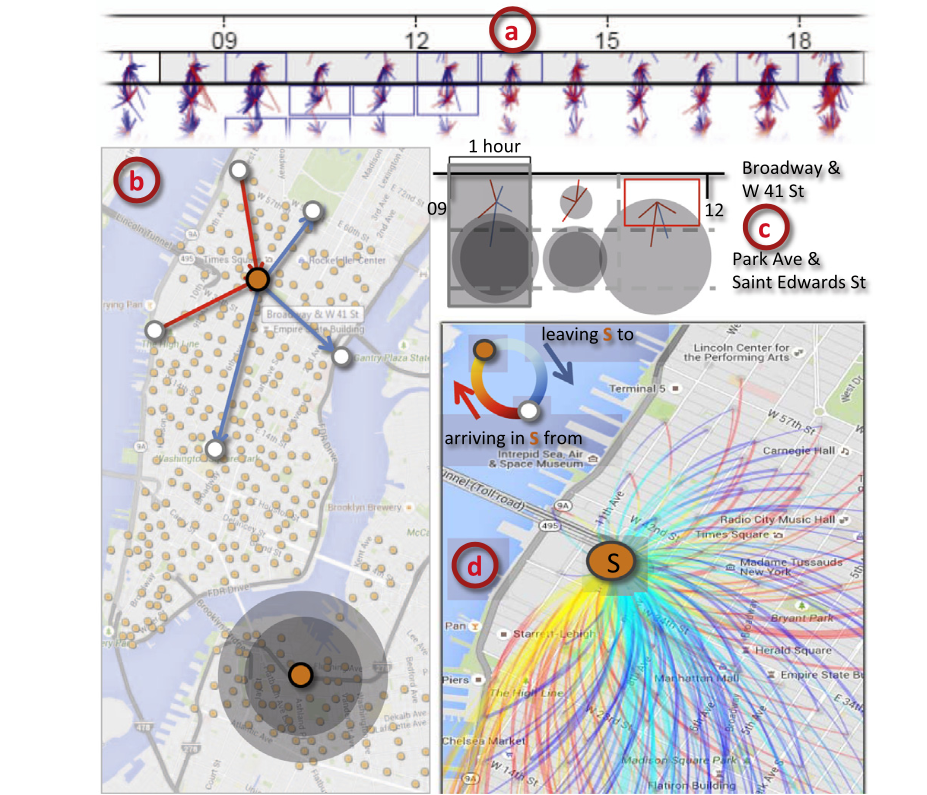
\includegraphics[scale=.3]{screenshot_article.png}
	\caption{Les différentes visualisations extraite de l'article \cite{Oli16}}
	\end{center}
	\end{figure}
	
	L’application proposée par les chercheurs est divisée en trois fenêtres principales.
	La première permet de naviguer sur une carte d’une ville. Elle permet de voir les
	stations et les trajets sélectionnés par l’utilisateur à partir de la fenêtre centrale.
	Cette dernière, est une matrice qui contient les trajets pour chaque station, sur une
	intervalle de temps, 24 heures ici. Elle permet de sélectionner avec la souris un
	ensemble de trajets pour une station donnée et une heure donnée, que nous appellerons glyphes.
	ce qui permet de sélectionner une plage horaire ou tous les trajets d'une station par exemple.
	La troisième fenêtre, située à droite, met a disposition un ensemble de filtre modifiable
	par des tirettes ou des cases à cocher. \\
	
	Les fonctionnalités et la manière de les utiliser ont été introduite dans la section
	d'introduction \ref{introduction}.\\

	Ce lien montre de quelle manière ils utilisent leur application pour afficher des trajets et
	des stations avec leur jeu de données. Cette vidéo est portée plus spécifiquement sur la manière
	de sélectionner des trajets.\\
	\url{https://drive.google.com/file/d/0B3aeg8yMfRj0MWFmUHZ6ZlR4MzA/view}\\
	Une impression écran a été faite à la figure \ref{fig:trips_screen}\\
	
	\begin{figure}[!h]
	\begin{center}
	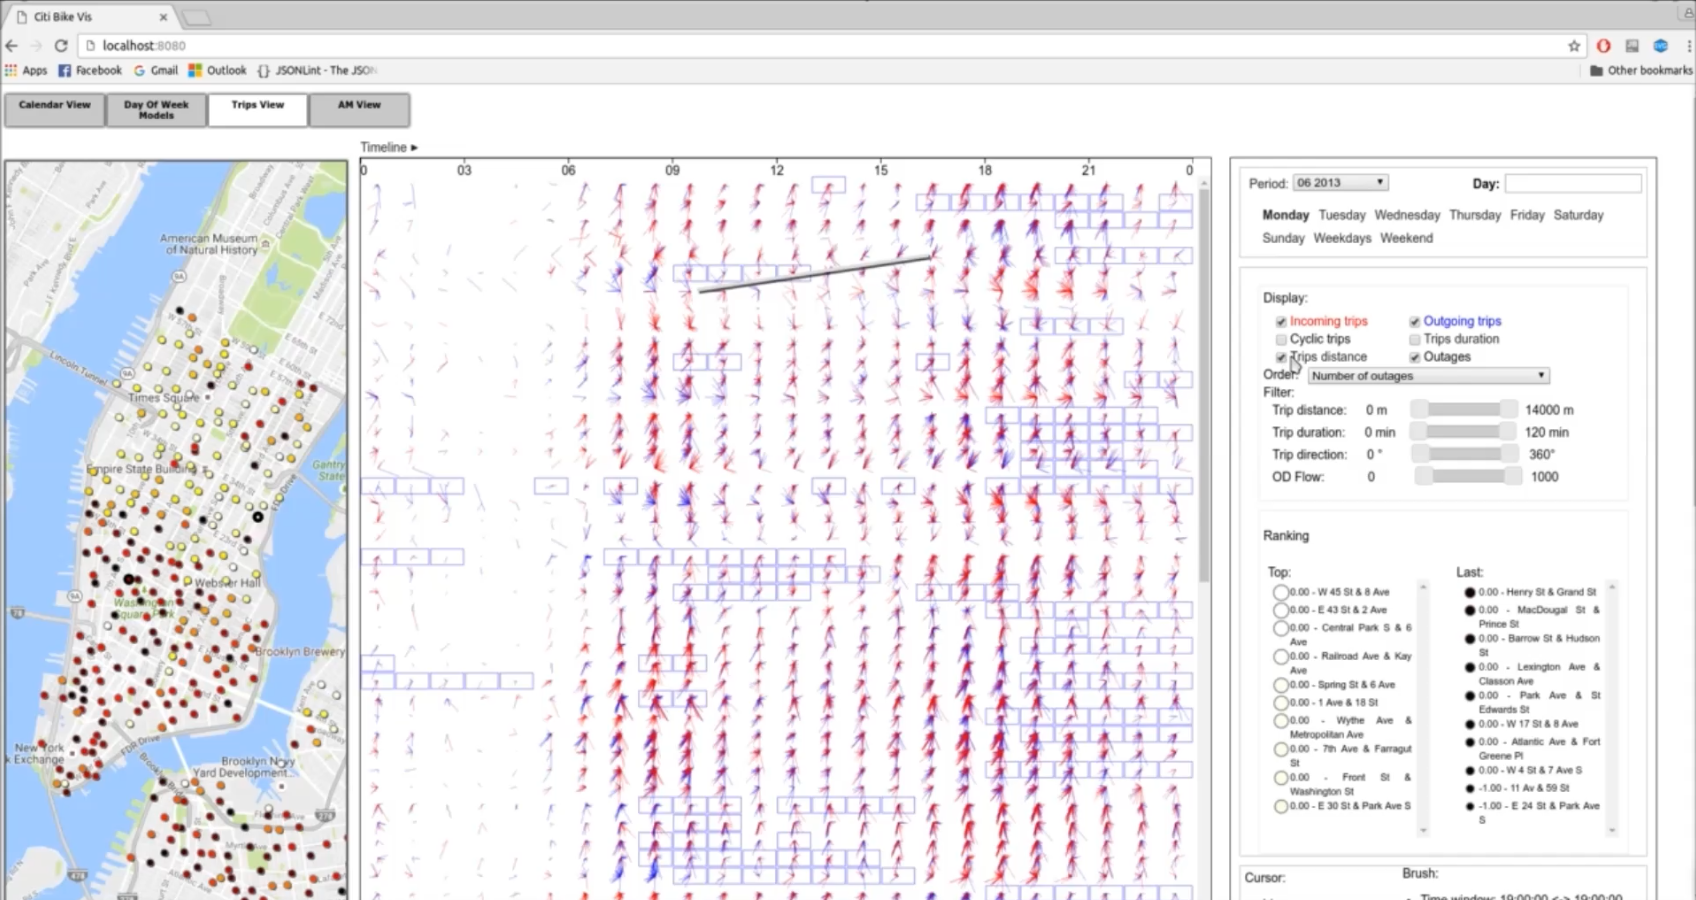
\includegraphics[scale=.3]{existant_trips.png}
	\caption{Impression écran du logiciel proposé par les chercheurs, visualisation des trajets}
	\label{fig:trips_screen}
	\end{center}
	\end{figure}
	
	Ce lien montre l'utilisation de
	Ces fonctionnalités ne feront développées dans notre application.\\
	\url{https://drive.google.com/file/d/0B3aeg8yMfRj0R3VKQjdtX1htUUU/view}\\
	Une impression écran a été faite à la figure \ref{fig:station_screen}\\
	
	\begin{figure}[!h]
	\begin{center}
	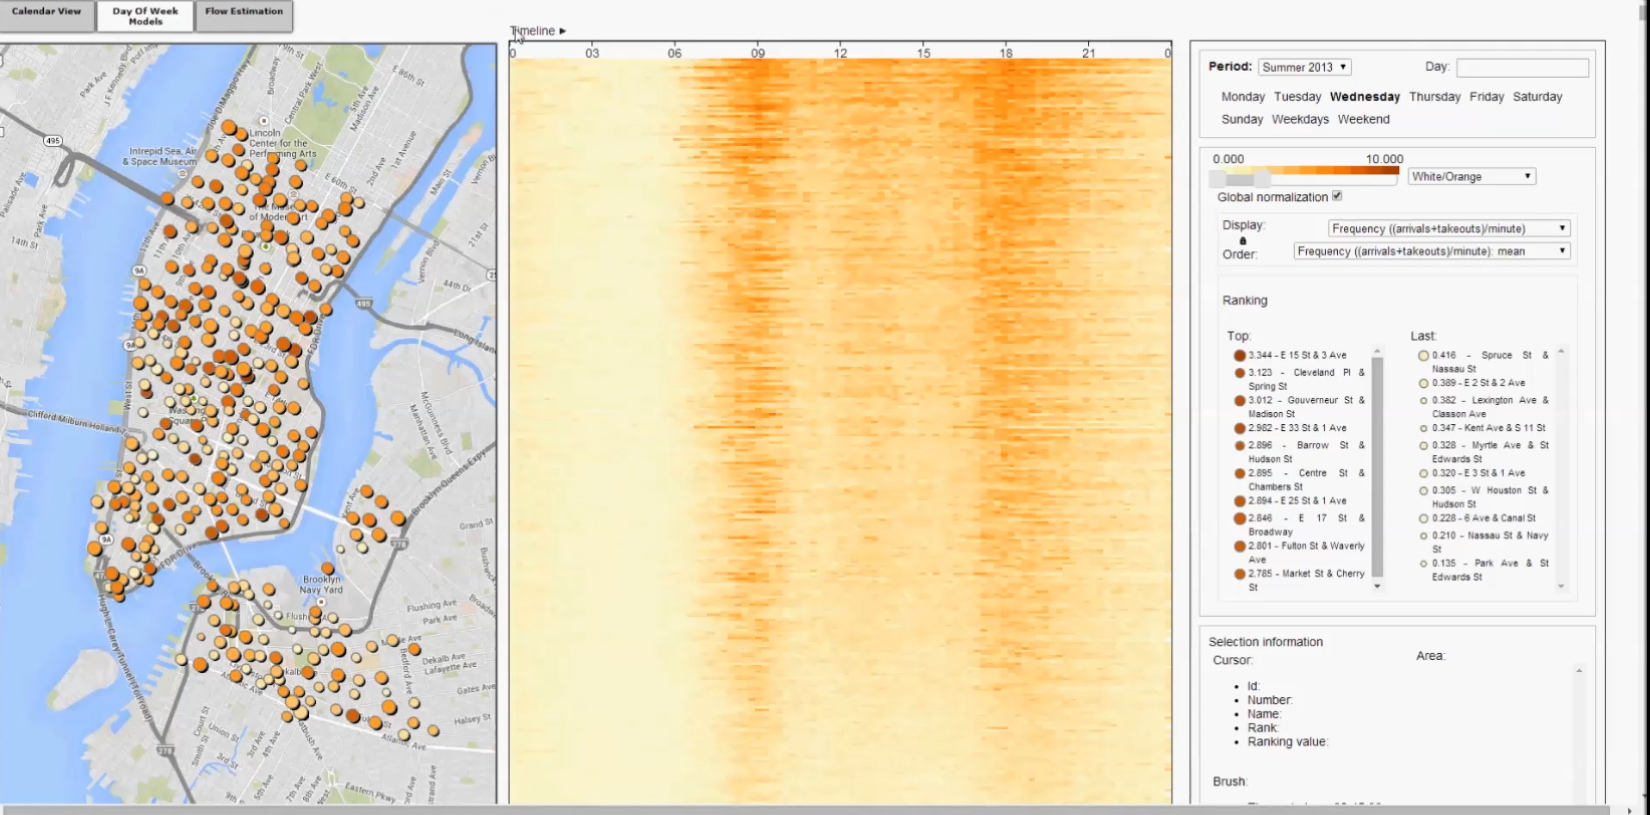
\includegraphics[scale=.3]{existant_station_state.png}
	\caption{Impression écran du logiciel proposé par les chercheurs, visualisation des états
	des stations}
	\label{fig:station_screen}
	\end{center}
	\end{figure}
	
	Quand on visionne la vidéo proposée par les chercheurs, on peut s'apercevoir dans un premier
	temps, qu'elle l’application est lancée depuis Google Chrome. Son URL* (localhost :8080)
	nous indique qu’il s’agit d’une démonstration en local. Ne pouvant pas tester l’application,
	nous avons peu d’informations sur sa rapidité en fonction du nombre de données et la manière
	précise de son fonctionnement. Aussi, nous ne savons pas à quoi correspondent les jours de la
	semaine dans la partie filtre. En revanche, on peut supposer que les performances ne
	sont pas optimales avec ce type de technologie pour le web (on peut constater
	quelques lenteurs dans ces vidéos).\\
	Comme expliqué précédemment, notre application a pour but de reprendre les
	fonctionnalités de cette application.
	
\newpage
	\section{Bibliographie}
		\begin{itemize}
			\item L'article \cite{Oli16} introduit clairement les problèmes rencontrés
			des systèmes de vélos en libre service. Notamment des problèmes d'équilibrage,
			de consommation de carburant pour les véhicules faisant la navette pour
			rééquilibrer les stations de vélos. On peut y puiser une grande source
			d'informations pour réaliser notre interface graphique. Ce sera le document sur
			lequel nous nous reposerons le plus.

			\item L'article \cite{Ali14} explique comment détecter les stations les plus
			connectées. Il donne un aperçu sur  l'utilisation des filtres (date, lieu, heure...).

			\item \cite{BC16} est un article sur les systèmes de partage de vélos. Il parle
			de l'application FunFEM qui permet de visualiser des données afin de juger de
			l'efficacité de ces systèmes.

			\item \cite{BSM17} est une application en ligne, qui permet de visualiser en
			temps réel des statistiques sur des bornes disponible dans une ville
			sélectionnée.  Elle indique également le nombre de vélos disponibles dans le
			monde en temps réel.

			\item L'article \cite{BW} de Ben Wellington, nous donne un bel aperçu sur la
			manière dont l'analyse statistique des données sur les utilisateurs du système de
			vélos en libre service peut être utilisée. Il montre comment les sociétés qui
			mettent à disposition les vélos dans la ville de New York pourraient augmenter
			leurs revenus grâce à une analyse des trajets des utilisateurs.

			\item \cite{JL} Recherches réalisées sur la manière d'optimiser l'équilibrage
			des stations de vélos en libre service. Un des problèmes avec les stations de vélos
			est la gestion de l'équilibrage du nombre de  vélos dans chaque station. Il explique
			comment prédire à l'aide de données un épuisement de vélos dans certaines stations.
			Ainsi, à l'aide d'analyses d'une multitude de données sur la météo ou l'âge des
			utilisateurs par exemple, il est possible de d'optimiser la répartition des vélos et
			de faire des prédictions.

			\item Vidéo postée par Oliveira G \cite{state_station}, qui présente l'interface
			graphique de l'application web. Les différentes visualisations sont principalement
			portées sur l'analyse statistique des stations dans une ville donnée.

			\item Vidéo postée par Oliveira G \cite{trips}, qui présente cette fois une
			interface portée sur l'analyse des trajets. On peut sélectionner différents types
			de filtres.

		\end{itemize}

\newpage
\part{L'analyse des besoins}
	\section{Besoins non fonctionnels}
		\subsection{Interfaces}
		Le texte de l’interface graphique sera en anglais.

		\subsection{Affichage des trajets}
		Les trajets seront affichés sur la carte par des courbes depuis le points de départ du
		trajet jusqu’au point d’arrivée.

		\subsection{Performances}
		Afin d’assurer la fiabilité du logiciel, des tests unitaires seront réalisés avec
		Banditcpp.\\
		"Bandit est un framework pour C++ 11 développé pour faire des tests unitaires. Bandit est
		l’en-tête seulement, donc il n’est pas nécessaire de compilation supplémentaire avant de
		pouvoir commencer à l’utiliser. Bandit a été testé avec les compilateurs suivants :
		GCC 4.5, GCC 4.6, GCC 4.7, GCC 4.8, Clang 3.2, VS2012.
		Bandit est sous licence libre MIT. \\
		Bandit est livré avec un projet cmake pour générer des auto-tests bandit."
		(\url{http ://www.banditcpp.org/})\\
	
		L’application devra en priorité, tourner aussi sur une carte NVIDIA, elle doit aussi,
		sur demande du client, s’exécuter sur une carte graphique Quadro K2000M. Ne 
		disposant pas de ce genre de carte, l'application sera testée sur une machine 
		disposant d'une carte graphique NVIDIA, puis sur la machine personnelle du client. \\
		
		On peut distinguer plusieurs attentes de rapidité en fonction des fonctionnalités :
		Lors de la lecture du fichier, le délai d’attente peut être long car il y a
		beaucoup de données à charger, on peut estimer ce délai à quelques secondes voire
		quelques minutes. \\
		
		Lors de l’application des divers filtres, le délai dois être assez court car l'utilisation
		de ces filtres est assez récurrente.
		Lors du déplacement sur la carte et donc du rafraîchissement des données de celle-ci,
		le programme doit tourner en temps réel et on ne doit pas sentir de latence lors du
		déplacement sur la carte. Le délai doit donc être très court (dans l’ordre des
		millisecondes).\\
		Le code devra être très bien documenté, pour cela on utilisera Doxygen.
		"Doxygen est l’outil standard de facto pour générer de la documentation à partir de
		sources C++ annotées, mais il prend également en charge d’autres langages de
		programmation populaires.\\
		Il peut générer un navigateur de documentation en ligne (en HTML) et/ou un manuel de
		référence hors ligne à partir d’un ensemble de fichiers sources documentés. Il est
		également possible de générer des résultats en format RTF (MS-Word), PostScript,
		PDF hypertexte, HTML compressé et pages de manuel Unix. La documentation est 
		extraite directement des sources, ce qui rend beaucoup plus facile de conserver
		la documentation conforme au code source. \\
		Doxygen est développé sous Mac OS X et Linux, mais est configuré pour être très
		portable."\\
		
		\url{http ://www.stack.nl/ dimitri/doxygen/index.html} \\
		
		La dernière version de Qt sera utilisée, à l’heure actuelle, c’est la version
		5.8 stable.\\
		Pour le rendu graphique, la version d’OpenGL doit être supérieure à la version 3.2.
		Ainsi, aucune fonction obsolète ne sera utilisée.\\
		Le code C++ sera compilable avec le compilateur g++ 4.9.
		
	\newpage
	\section{Besoins fonctionnels}
		\subsection{Visualisation de la carte de la ville}
		Une fenêtre sur la partie gauche sera dédiée pour visualiser les trajets de
		manière géographique avec une carte.\\
		La carte d’une ville pourra être chargée avec OpenStreetMap\\
		La carte affiche uniquement les stations de la ville lorsqu’il y a des stations
		sélectionnées dans la matrice de chronologie, elle n’affiche que celles-ci (ainsi
		que les trajets qui y sont associés).\\
		Les trajets sont dessinés par des courbes avec un dégradé de deux couleurs.\\
		Les départs sont dessinés du cyan (station d’origine) vers le bleu (station de
		destination) dans le sens horaire.\\
		Les arrivées sont dessinées du rouge (station d’origine) vers le jaune
		(station de destination) dans le sens anti-horaire.\\
		Lorsque l’utilisateur passe sa souris sur une station de la carte, la ligne associée
		à la station est surlignée en noir dans la matrice de chronologie des trajets.\\
		Lorsque l’utilisateur passe sa souris sur une station de la matrice de chronologie
		des trajets, la station est surlignée en noir sur la carte.\\
		L’utilisateur pourra faire un zoom avant ou un zoom arrière grâce à la molette de la
		souris.\\
		Il pourra aussi se déplacer dans la carte, à gauche, à droite, en haut et en bas. Il
		réalisera cette action soit en appuyant sur des boutons, soit grâce à un système
		de glisser/déposer, afin de permettre une translation et se déplacer dans la carte.\\
		
		\subsection{Matrice de la chronologie des trajets}
		Axe horizontal : temps en heure (une colonne pour chaque heure)\\
		Axe vertical : stations (une ligne pour chaque station) les stations sont représentées dans
		des cellules par des petites étoiles (les lignes étant les trajets, représentés
		avec leurs directions et leur longueur)\\
		Arrivées en rouge\\
		Départs en bleu\\
		Trajets cycliques par des cercles transparents dont le rayon est proportionnel à
		la distance du trajet\\
		Possibilité de sélectionner les stations avec la souris, selon un intervalle horaire
		Les stations sélectionnées dans cette fenêtre sont visibles sur la carte, avec
		les trajets qui y sont associés\\
		Possibilité de dérouler, sur 24 heures, l’activité des emprunts des vélos
		en lançant l’animation (en appuyant sur le bouton play)\\
		
		\subsection{Interface de sélection des filtres}
		Possibilité de pouvoir filtrer dans le temps\\
		Un mois et son année : menu déroulant avec choix chargés à partir de fichiers
		données\\
		Un jour précis : entrée du jour du mois (un entier compris 1 et 31) dans un champ
		de texte\\
		Jour de la semaine/jours ouvrés/weekend\\
		Possibilité de filtrer selon les propriétés des trajets\\
		Arrivées : si cochée, affiche (en rouge) les trajets arrivants, sur la carte ainsi
		que dans la chronologie des trajets\\
		départs : si cochée, affiche (bleu) les trajets partant, sur la carte ainsi que
		dans la chronologie des trajets\\
		trajets cycliques : si cochée, affichés (par un cercle gris transparent dont le
		rayon est proportionnel à la longueur du trajet) les trajets cycliques, dans la
		chronologie des trajets\\
		durées des trajets : si cochée, prend en compte la durée des trajets\\
		longueurs des trajets : si cochée, prend en compte la longueur des trajets
		(les longueurs des traits des trajets dans chaque cellule de la chronologie des
		trajets sont relatives au trajet le plus long), sinon, tous les traits sont
		de même longueur\\
		
		Filtrer selon des valeurs entières comprises dans un intervalle borné par une
		valeur minimale et une valeur maximale:
		\begin{itemize}
			\item[•]longueur (en mètres)
			\item[•]durée (en secondes)
			\item[•]direction (en degrés)
			\item[•]flux d’origine-destination
		\end{itemize}
	
	\newpage
	\section{Scénarios}
	
	\newpage
	\section{Prototype}
	Pour la remise de la 1er version, nous avons voulu de rendre un programme qui permettait
	d'afficher des stations et des trajets ainsi qu'un aperçu de ce que cela pourrait rendre
	dans la timelinematrix. Ayant un temps très court pour réaliser cela, nous avons testé
	d'afficher ces éléments avec les objets que \href{https://www.qt.io/}{Qt5}
	nous met à disposition.\\
	

	\begin{figure}[!h]
	\begin{center}
	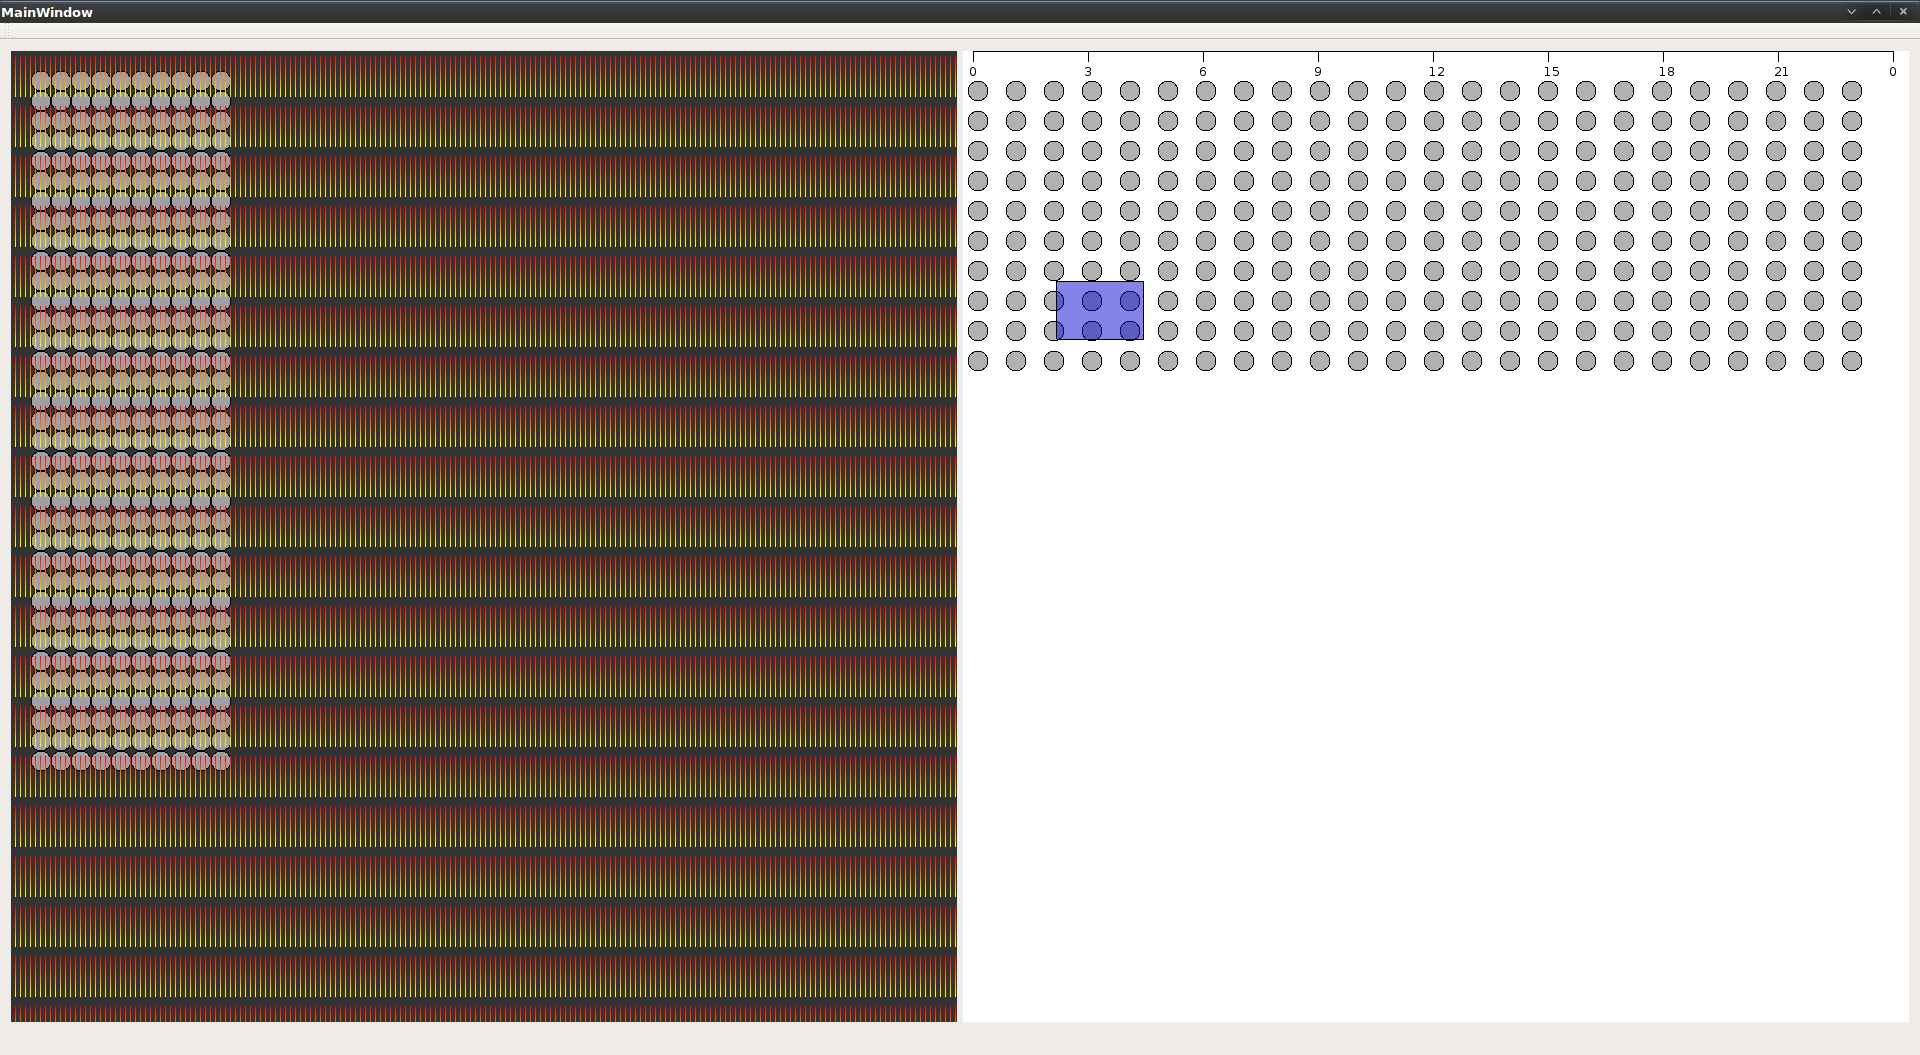
\includegraphics[scale=0.2]{prototype1_screen_shot.png}
	\caption{Prototype de la première version}
	\end{center}
	\end{figure}		
	
	Ce prototype nous a permis de nous rendre compte que l’utilisation des objets
	\href{https://www.qt.io/}{Qt} pour dessiner les trajets et stations
	ne satisfera pas les attentes des besoins non fonctionnels. C’est la raison pour
	laquelle, malgré les difficultés rencontrées nous avons quand même utilisé
	\href{https://www.khronos.org/registry/OpenGL-Refpages/gl4/}{OpenGL}
	pour le rendu.\\
	
	Des tests de performances ont été réalisés sur ce prototype et se trouve plus bas à la
	section \ref{tests_performances} sur les tests\.\\

\newpage
\part{L'architecture}

	\section{Architecture générale}
		\subsection{Architecture 3-tiers}
		\begin{figure}[!h]
		\begin{center}
		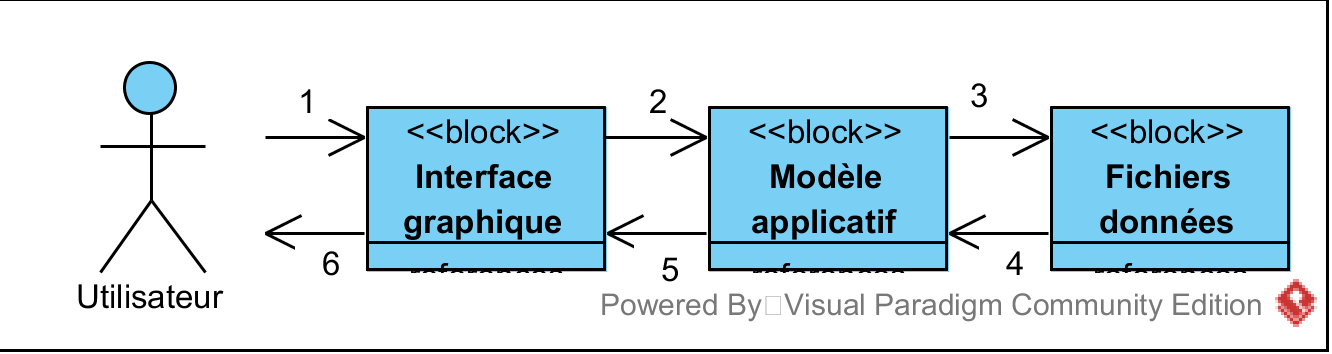
\includegraphics[scale=1]{dia_block_3tiers.png}
		\caption{Architecture 3-tiers}
		\end{center}
		\end{figure}
		
		L’architecture se compose de trois couches :
		\begin{itemize}
			\item[•]couche présentation
			\item[•]couche métier 
			\item[•]couche accès aux données\\
		\end{itemize}
			
		\begin{enumerate}
		\item L'utilisateur manipule le logiciel avec les contrôles (boutons, sliders à deux
		poignées et menu déroulant) de l’interface graphique. Ce seront, concrètement,
		des opérations de filtrages et de sélection des trajets, ainsi que de filtrage
		et de tri des stations. C’est dans cette couche que ces opérations sont appelées.\\
		
		\item Le contrôleur de l’interface manipule les données du modèle. C’est dans cette
		couche que les opérations demandées par l’utilisateur au 1) sont exécutées.\\
		
		\item (dans notre cas, le modèle n’écris pas sur les données, l’accès des données se
		fait en lecture seule)\\
		
		\item Le modèle accède aux données. Ici, le modèle ne fait que parser des fichiers,
		sans les modifier. Le fichiers sont refermés une fois l’opération de parsing
		terminée. Le modèle charge les données en initialisant une liste pour les trajets,
		une autre pour les stations. Cela se fait à chaque fois que l’utilisateur
		souhaite charger un fichier.\\
		
		\item Le modèle notifie l’interface graphique des résultats des opérations demandées
		depuis 1). Tous les composants graphiques concernés sont mis à jour, notamment la
		map affichant les trajets, ainsi que la matrice de chronologie des trajets.\\
		
		\item L’interface graphique affiche à l'utilisateur les résultats de ses requêtes.\\
		\end{enumerate}

		\subsection{Le design pattern MVC}		
		\begin{figure}[!h]
		\begin{center}
		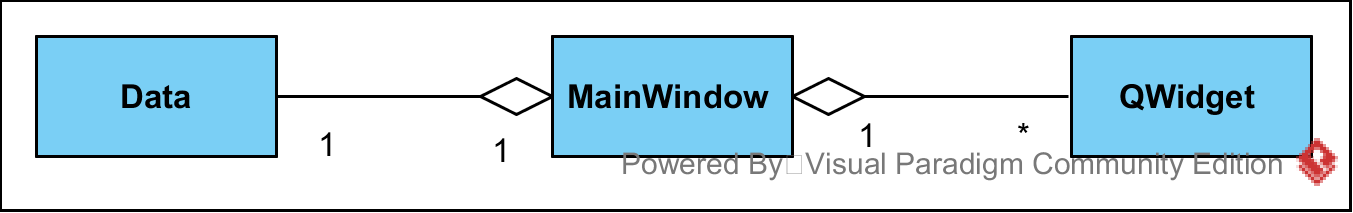
\includegraphics[scale=1]{dia_class_mvc.png}
		\caption{Relation des compositions des classes implémentant le MVC}
		\end{center}
		\end{figure}		
		
		L’architecture du projet est basée sur le design pattern MVC classique
		(Modèle/Vue/Contrôleur).\\
		
		\textbf{Le Modèle}\\
		Cette classe ne fait
		que contenir des données (les stations et les trajets), avec la possibilité de les
		charger à partir de fichiers texte, et les décharger. C’est elle qui gère
		l’allocation mémoire de ces données, ainsi que leur accès en lecture seule.\\
		
		\textbf{La Vue}\\
		C’est l’ensemble des composants de l’interface graphique (les widgets). Ces widgets
		sont implémentés par Qt soit en C++, soit en QML (pour Qt Modeling Language). Il sont
		contenus dans la classe “MainWindow”.\\
				
		\textbf{Le Contrôleur}\\
		C’est la classe “MainWindow”, nom généré par le designer d’interface graphique de
		QtCreator. Elle est contenue dans l’espace de nom “Ui” (également généré par Qt).
		Elle joue le rôle de contrôleur en étant composée des composants graphiques ainsi que
		du modèle. Elle fait communiquer le Modèle et la Vue via le mécanisme des signaux
		implémenté par Qt.\\
			
		\subsection{Les packages}
		\begin{figure}[!h]
		\begin{center}
		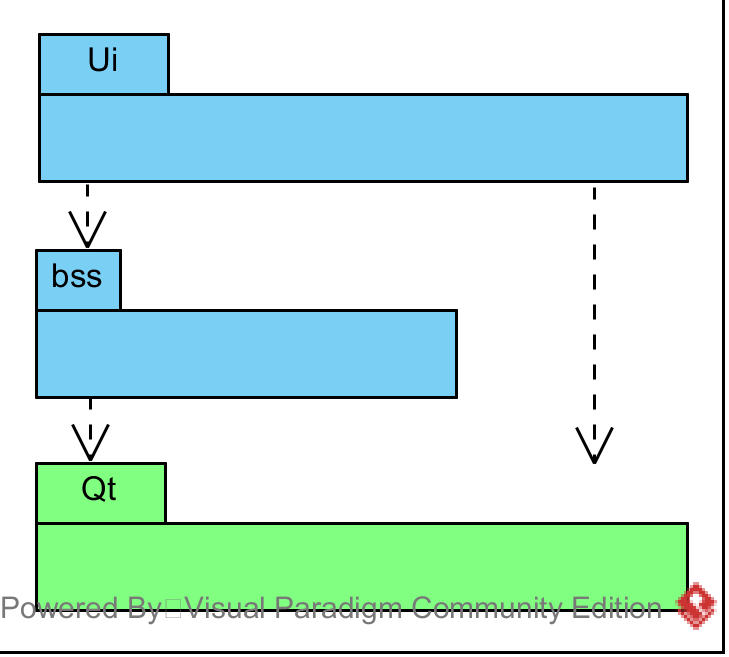
\includegraphics[scale=1]{dia_package.png}
		\caption{Diagramme de package}
		\label{fig:dia_package}
		\end{center}
		\end{figure}		
		
		On distingue deux espaces de noms (voire trois si on considère que les classes de
		Qt sont contenues dans un espace de nom) (cf. Figure: \ref{fig:dia_package} Diagramme de
		package):\\
	
		\begin{itemize}
		\item[•] l’espace de nom “Ui” (pour “User interface”), qui est généré par Qt.
		Il est utilisé pour y regrouper les composants graphiques qui sont auto-générés avec
		le designer d’interfaces graphiques. Le Contrôleur est également contenu dans “Ui”.
		La Vue et le Contrôleur sont donc gérés au niveau de “Ui”. “Ui” dépend de “bss” et des
		classes de Qt.\\
		
		\item[•]l’espace de nom “bss” (pour “Bike Sharing System”), qui contient les classes
		du Modèle. “bss” utilise des objets et des fonctions de Qt en plus de ceux proposés
		par C++ 14.
		\end{itemize}

\clearpage
\newpage
\part{Code}
	\section{Interface graphique}
	L’interface graphique a été créée avec designer intégré à Qt Creator : le QtDesigner. Il permet de créer rapidement une interface d’application desktop avec le drag and drop (c’est le principe d’un éditeur WYSIWIG : “what you see is what you get”). Au départ, l’éditeur présente une fenêtre principale vide. L’interface se construit en y ajoutant les widgets : les composants de l’interface.

	L’interface utilisateur est composée de 3 fenêtres :\\
	\begin{itemize}
	\item[•] la fenêtre à gauche permet, après le chargement des données, d’obtenir une représentation géographique des trajets.
	\item[•] la fenêtre au milieu permet de voir les trajets de manière statistique, représentés sous la forme de matrice.
	\item[•] la fenêtre à droite est celle des contrôles. Elle permet d’appliquer des filtres sur les trajets selon différents paramètres comme la date, la distance, etc, et de trier les stations.
	\end{itemize}
	
		\subsection{Premier prototype}
		\begin{figure}[!h]
		\begin{center}
		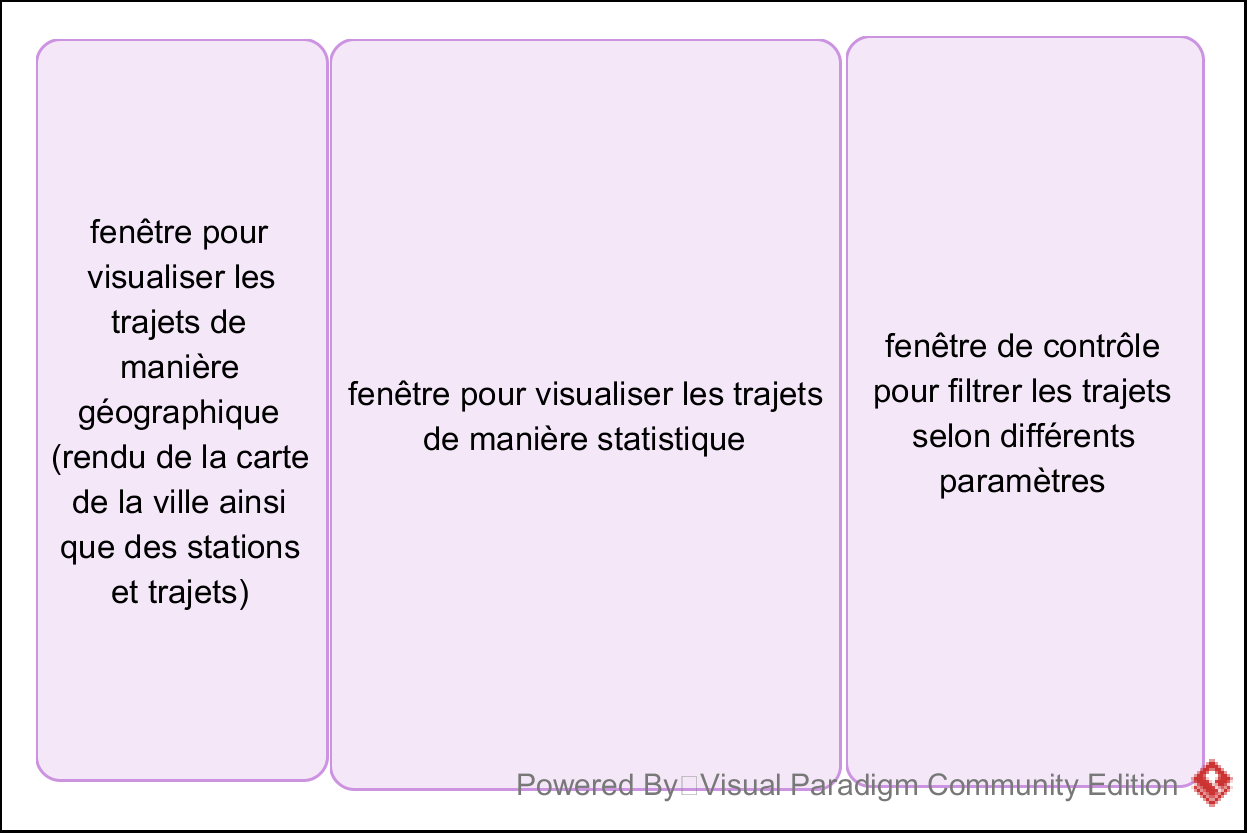
\includegraphics[scale=1]{dia_proto-interface_1.png}
		\caption{Premier prototype d’interface graphique}
		\end{center}
		\end{figure}
		
		La figure ci-dessus illustre un premier prototype d’interface graphique. Il décompose l’interface en 3 parties distinctes, celle du milieu étant la plus large, celles des extrémités étant de largeur à peu près égales.
		
		\subsection{Second prototype}
		\begin{figure}[!h]
		\begin{center}
		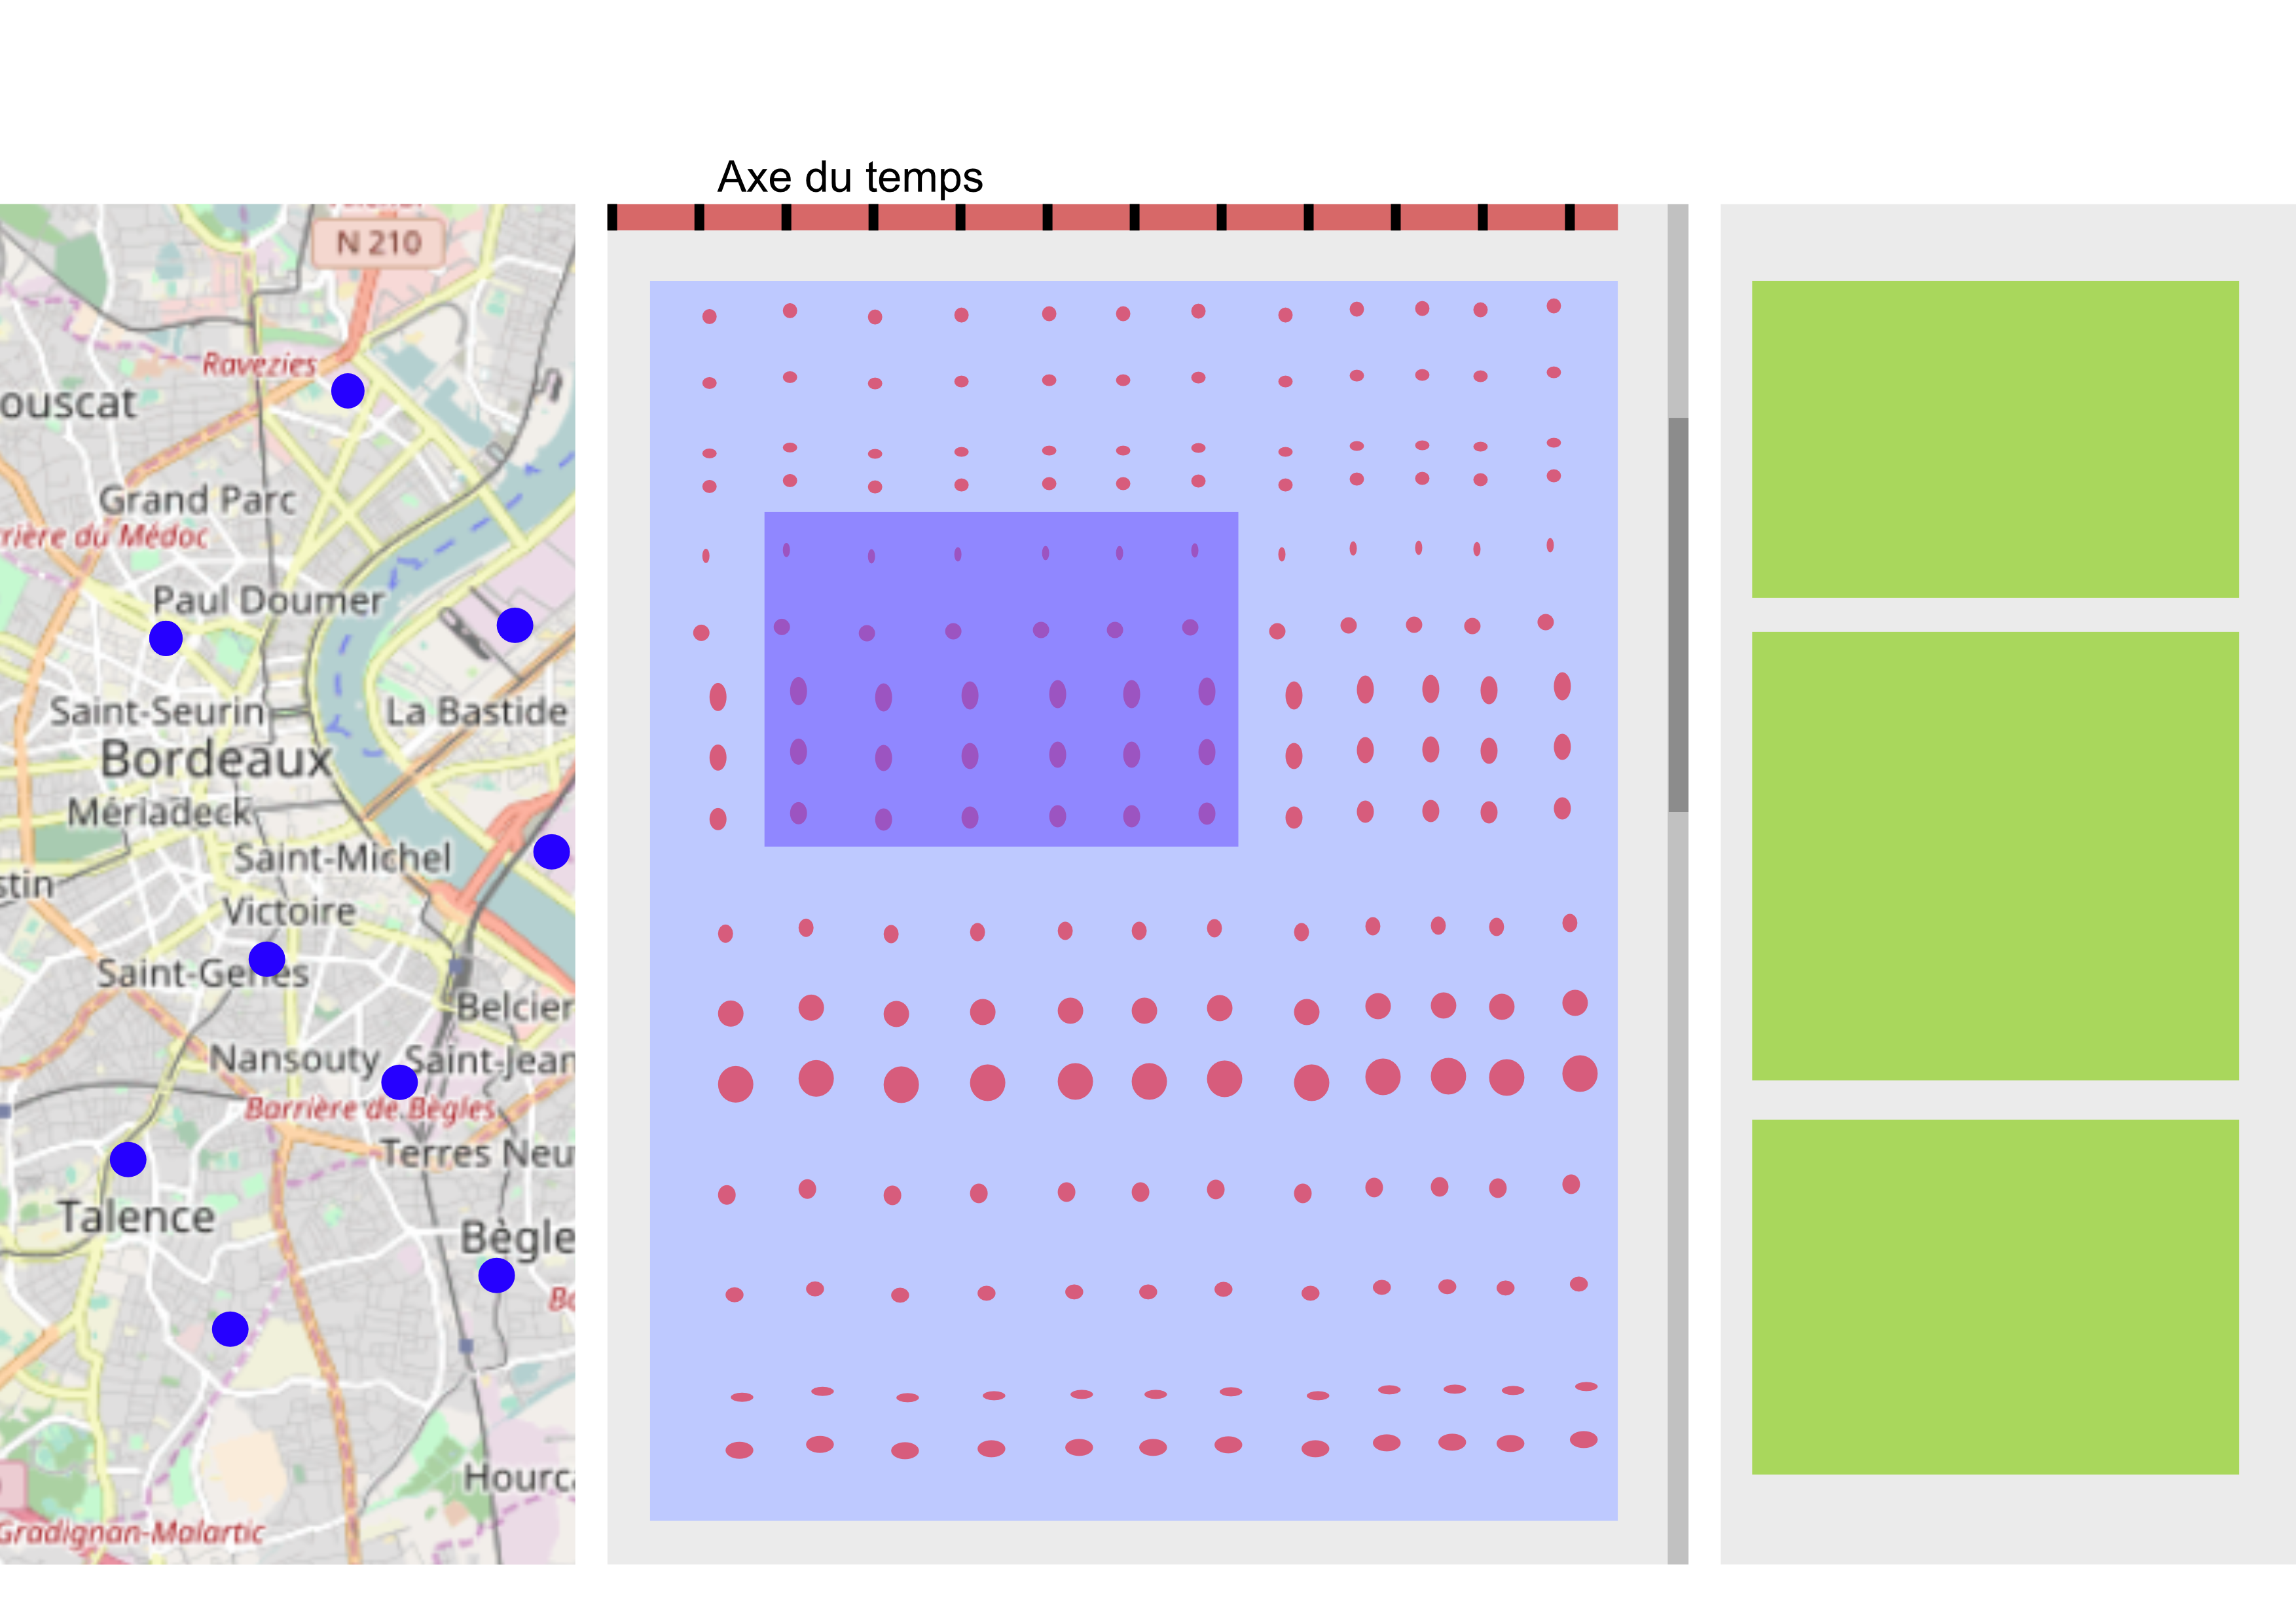
\includegraphics[scale=.5]{dia_proto-interface_2.png}
		\caption{Second prototype d’interface graphique}
		\label{fig:proto_int_2}
		\end{center}
		\end{figure}
		
		La figure \ref{fig:proto_int_2} montre une évolution de l’interface, notamment :\\
		\begin{itemize}
		\item[•] la fenêtre de gauche contient une map (en l'occurrence celle de Bordeaux), avec représentées en bleu les stations (celles-ci sont fictives).
		\item[•] la fenêtre au centre représente une matrice (tableau bi-dimensionnel) de disques. L’axe horizontal représente le temps en heure, l’axe vertical celui des stations. Ces disques sont composés de trajets (chaque trajet formant une ligne de couleur bleue ou rouge, dessiné dans la direction du trajet). Il y a de nombreux trajets à représenter ce qui explique pourquoi ils sont représentés ainsi. Un disque montre donc tous les trajets pour une stations donnée, pour une heure de départ donnée. Enfin, il faut noter la présence d’une barre de défilement sur la droite, afin de parcourir les stations sur l’axe vertical.
		\item[•] la fenêtre de droite est découpée en trois parties.
		\end{itemize}
		
		
		\subsection{Release non-finale}
		
		Dans cette version non-finale de l’interface graphique (cf. Figure \ref{fig:screen_final_1}), on peut voir apparaître : \\
		
		\begin{figure}[!h]
		\begin{center}
		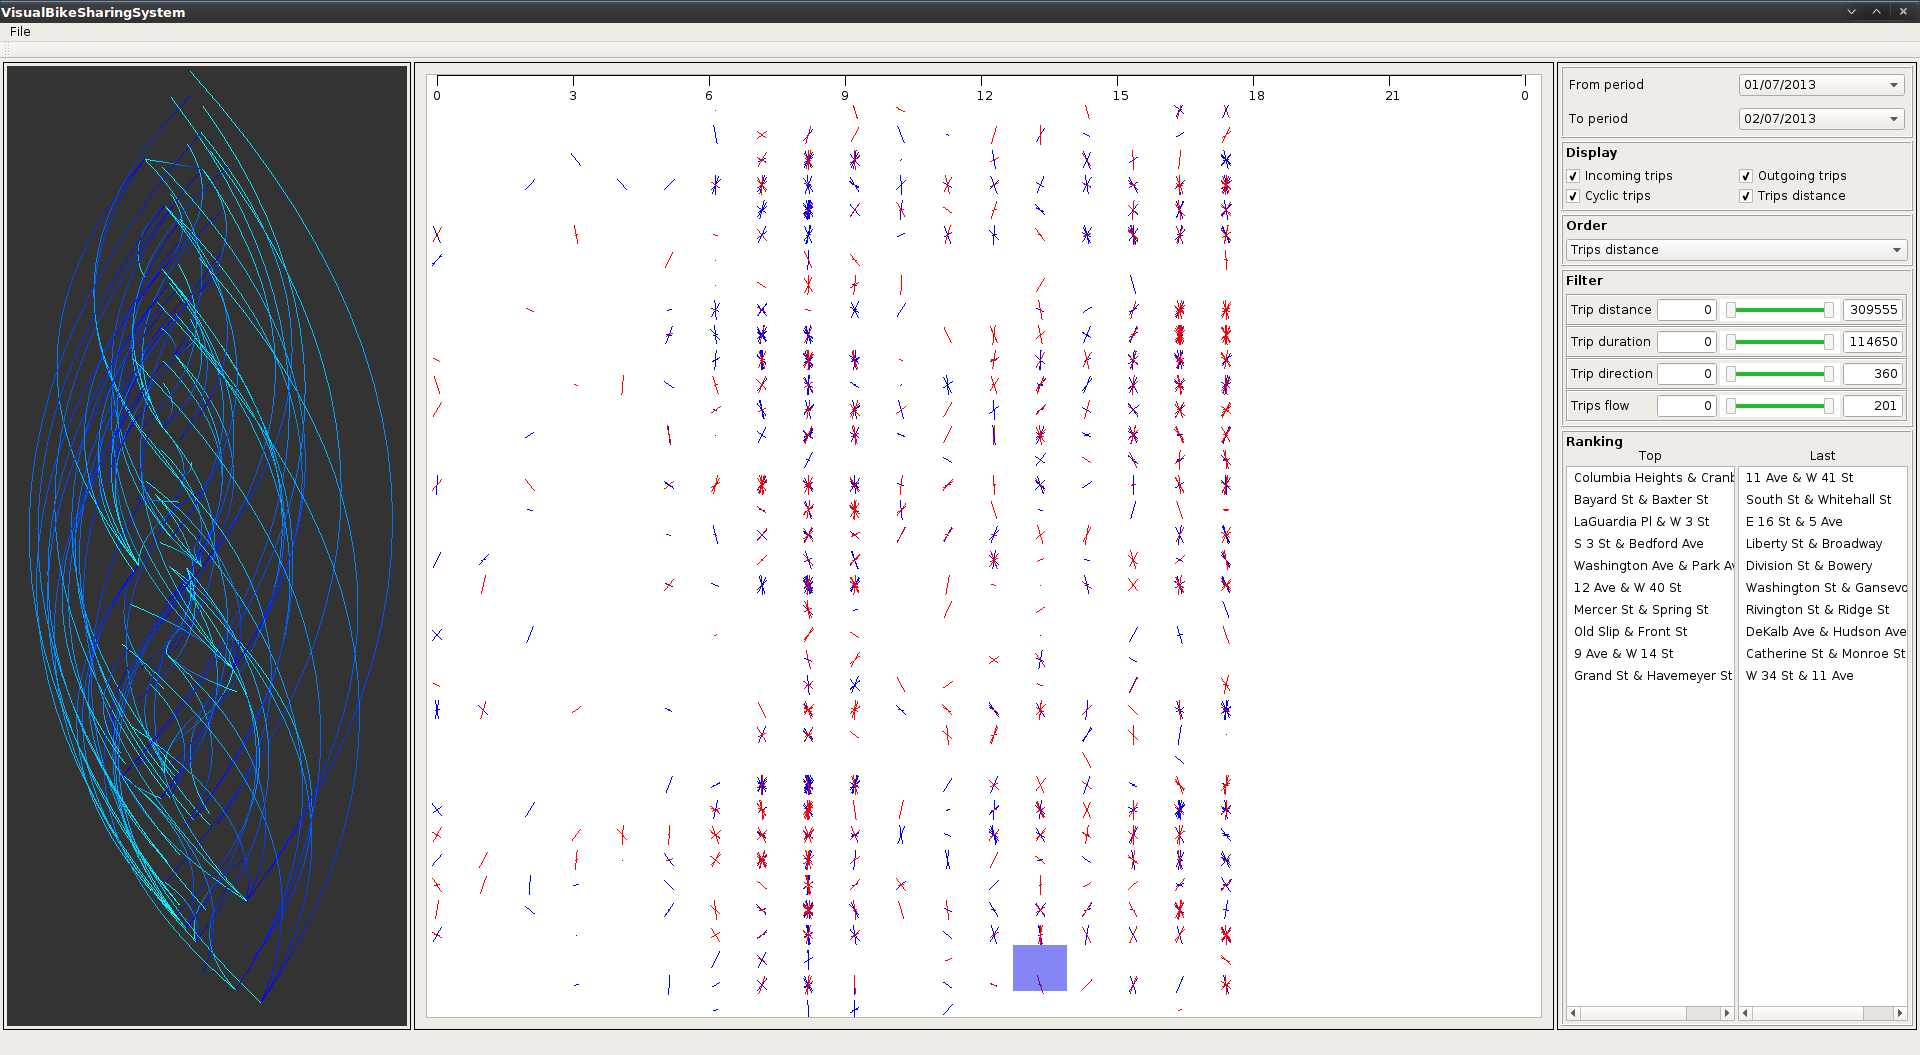
\includegraphics[scale=.25]{screen_final_1.png}
		\caption{Capture d’écran du programme en utilisation}
		\label{fig:screen_final_1}
		\end{center}
		\end{figure}
		
		\begin{itemize}
		\item[•] sur la fenêtre de gauche, les trajets sélectionnés sont affichés par des courbes dont la couleur est interpolée du bleu vers le cyan, pour les départs. Il est possible de défiler la map avec la souris, et de modifier le zoom avec la molette.
		\item[•] sur la fenêtre au centre, la matrice de chronologie des trajets dessine les “glyphes” (terme utilisé par l’article pour désigner un ensemble de petits traits, dirigés selon l’azimut du trajet). Un glyphe représente l’ensemble des trajets filtrés pour une stations donnée (la ligne) pour une heure donnée (la colonne). Au dessus de la matrice, il y a un label pour indiquer l’axe du temps, par intervalle de trois heure, allant de 0 à 24h. Il est possible de défiler sur les deux axes, ainsi que de sélectionner des trajets avec la souris (avec un mouse-drag classique). Le rectangle de sélection est dessiné en bleu
		\item[•] sur la fenêtre à droite, les contrôles pour traiter les données. Il est possible de filtrer les trajets sur leur date de départ avec des menus déroulants (tout en haut). Les cases à cocher juste en dessous permettent de spécifier des paramètres d’affichage des trajets selon leur type (arrivées, départs, cycles). Le menu déroulant, plus bas, permet de trier les stations. Puis, les quatre tirettes (ou sliders) à deux poignées définissent des intervalles pour filtrer les trajets (pour les trois premiers sliders) et filtrer les stations (pour celui tout en bas). Enfin, la section “Ranking” affiche les premières (à gauche) et dernières (à droite) stations après les avoir trié selon une propriété
		\end{itemize}
		
		Il faut également noter la présence d’un barre de menu, juste au dessus de la carte, avec la section “File” qui permet d’ouvrir et fermer des fichier données.\\

		Il faut aussi noter que les contrôles sont désactivés lorsqu’une opération estimée coûteuse est en cours d'exécution. Il sont rétablis lorsqu’elle prend fin.\\

		Enfin, chaque widget affiche une infobulle pour guider l’utilisateur lorsque la souris flotte sur le widget.

		\subsection{Release finale}
		
		\begin{figure}[!h]
		\begin{center}
		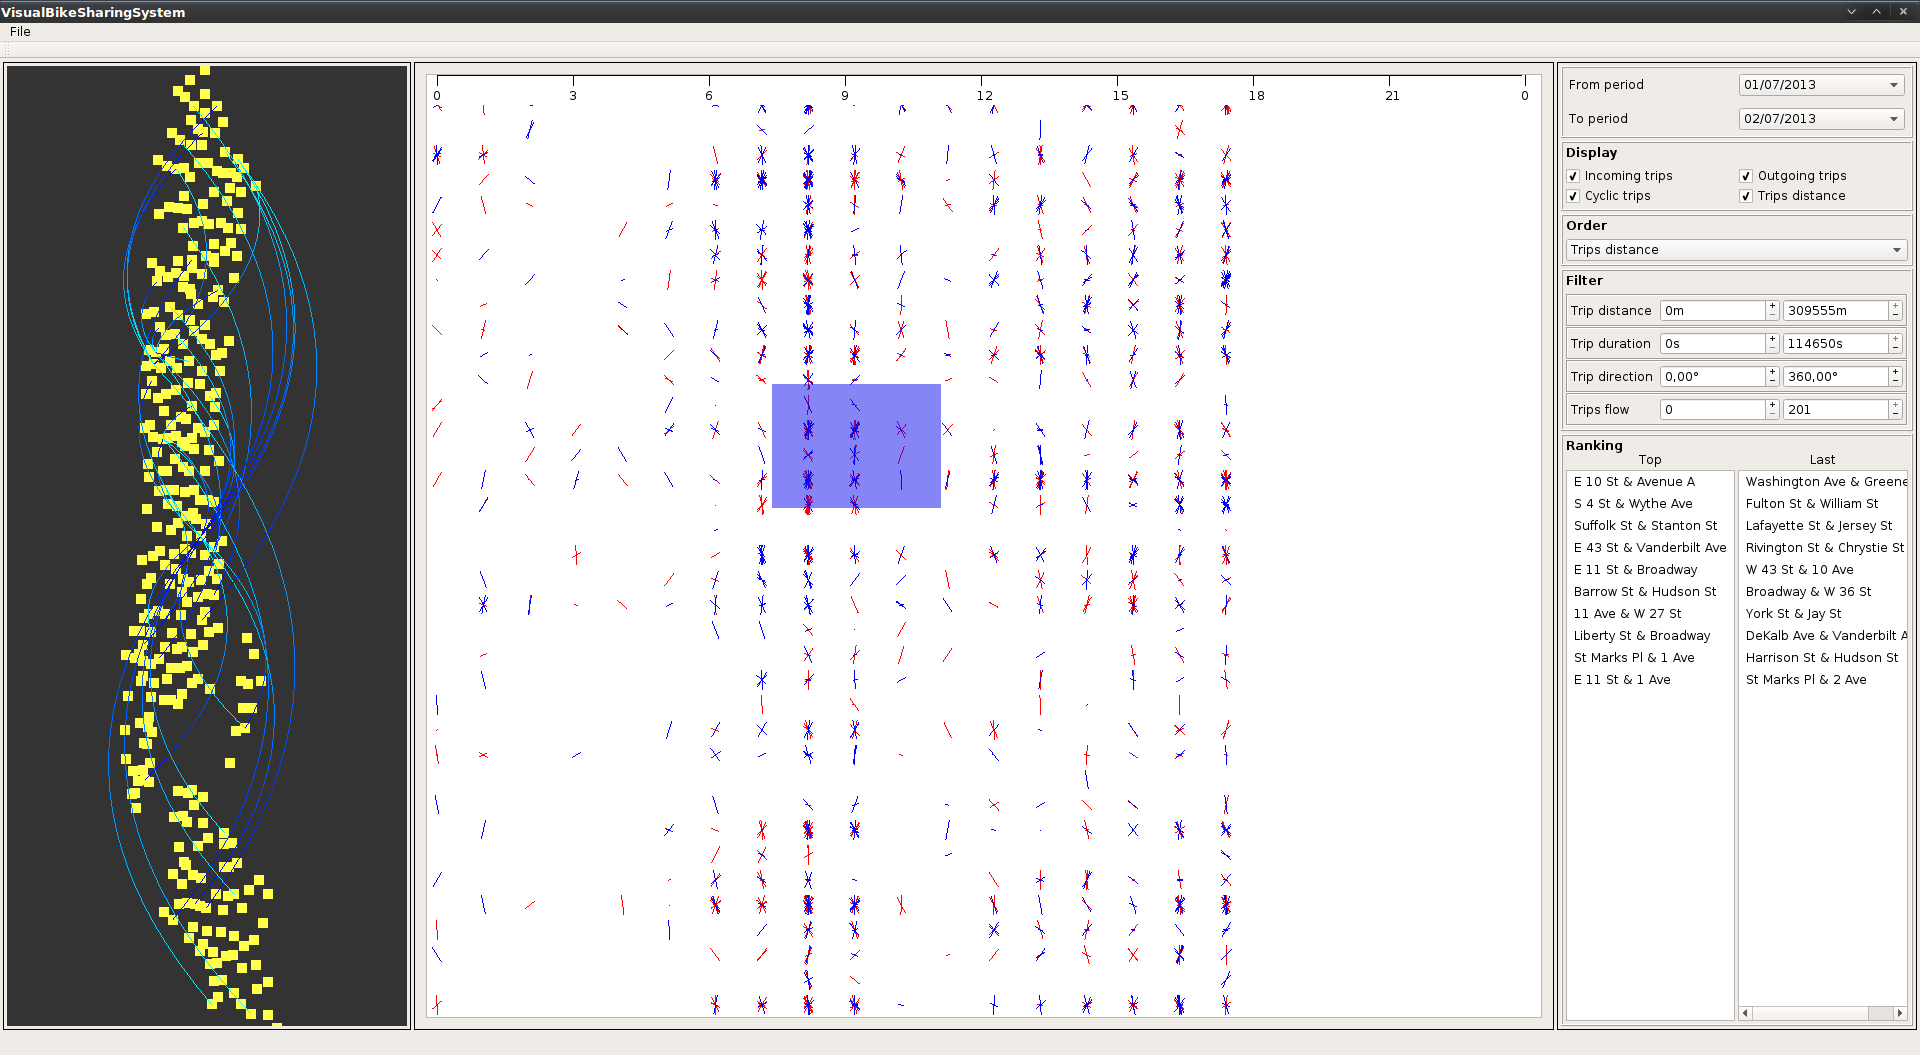
\includegraphics[scale=.25]{screen_final_2.png}
		\caption{Capture d’écran de la version finale du programme}
		\end{center}
		\end{figure}
		
		L’interface est sensiblement similaire à celle de la version finale, excepté que les sliders à deux poignées ont été remplacées par des spinboxes. La raison est que les sliders à deux poignées sont implémentés avec QtQuick (une librairie de widgets) et QML (Qt Modeling Language, proche du CSS). Leur utilisation nécessite donc des dépendances de librairies supplémentaires. Cela a été problématique pour le client qui n’avait pas installé ce module. De plus, le comportement de ces sliders était instable et buggé. Une autre solution aurait d'implémenter le slider à deux poignées avec C++ et OpenGL, mais nous n’avions pas le temps ni les compétences nécessaires.
		

	\newpage
	\section{Implémentation}
		\subsection{Le contrôleur (classe \textit{MainWindow})}
		\begin{figure}[!h]
		\begin{center}
		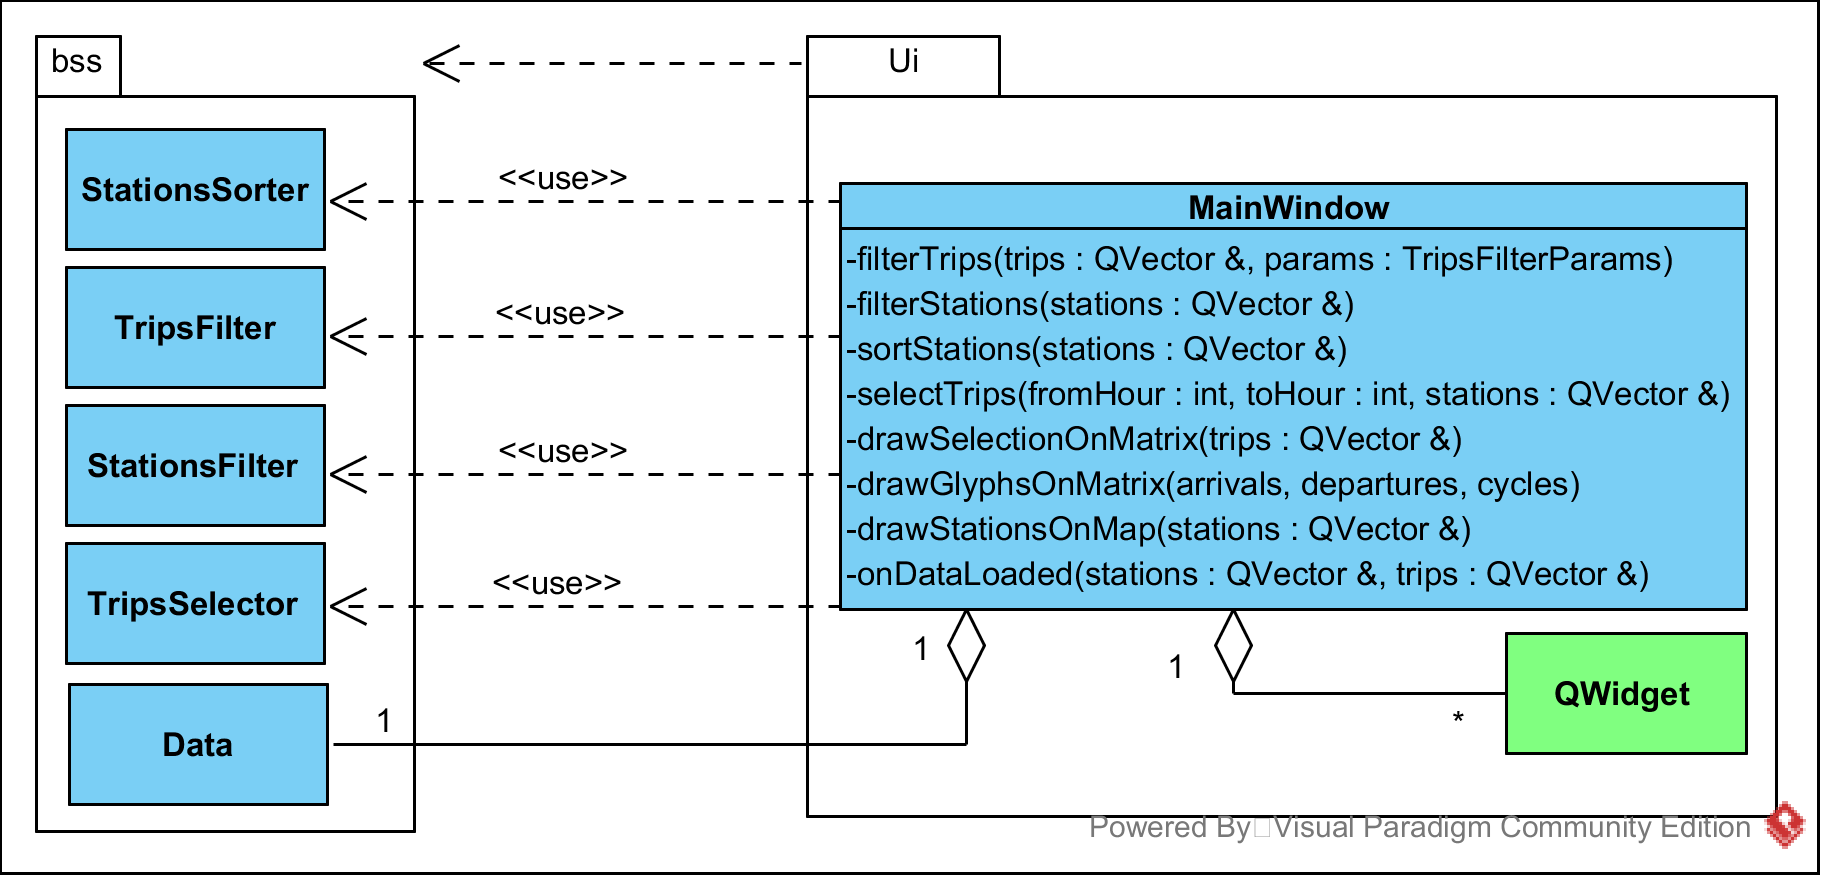
\includegraphics[scale=1]{class_diagram_controleur.png}
		\caption{Diagramme de classe du contrôleur, avec ses fonctions et usages principaux}
		\label{fig:dia_controleur}
		\end{center}
		\end{figure}
					
		C’est la classe principale. C’est un \textit{QObject} en héritant de la classe \textit{QMainWindow}.Elle implémente donc les fonctionnalités de réception et d’émission de signaux. C’est elle qui commande le modèle et la vue, en étant composée d’un objet de type \textit{Data}, et de l’ensemble des widgets de l’interface graphique. Elle dispose de nombreuses fonctions, notamment celle qui réagissent aux signaux émis par la vue et le modèle. Elle fait également usage des objets permettant le traitement des données, à savoir un \textit{StationsSorter} pour trier les stations et un \textit{StationsFilter} pour les filtrer, selon les propriétés de station, un \textit{TripsFilter} pour trier les trajets et un \textit{TripsSelector} pour les sélectionner, selon les propriétés des trajets (cf. Figure \ref{fig:dia_controleur}).\\
	
	Enfin, il n’est pas indiqué sur le schéma que \textit{MainWindow} entretient les listes des identifiants des données traitées (dans des \textit{QVector}) : un conteneur des identifiants des trajets filtrés, un autre pour ceux qui sont sélectionnés, et enfin un dernier pour les identifiants des stations filtrées et triées. Il est important de noter que l’ensemble des trajets sélectionnés doit appartenir à l’ensemble des trajets filtrés : la sélection se fait parmi les trajets filtrés.
		
		\subsection{Ouverture de fichiers}
		\begin{figure}[!h]
		\begin{center}
		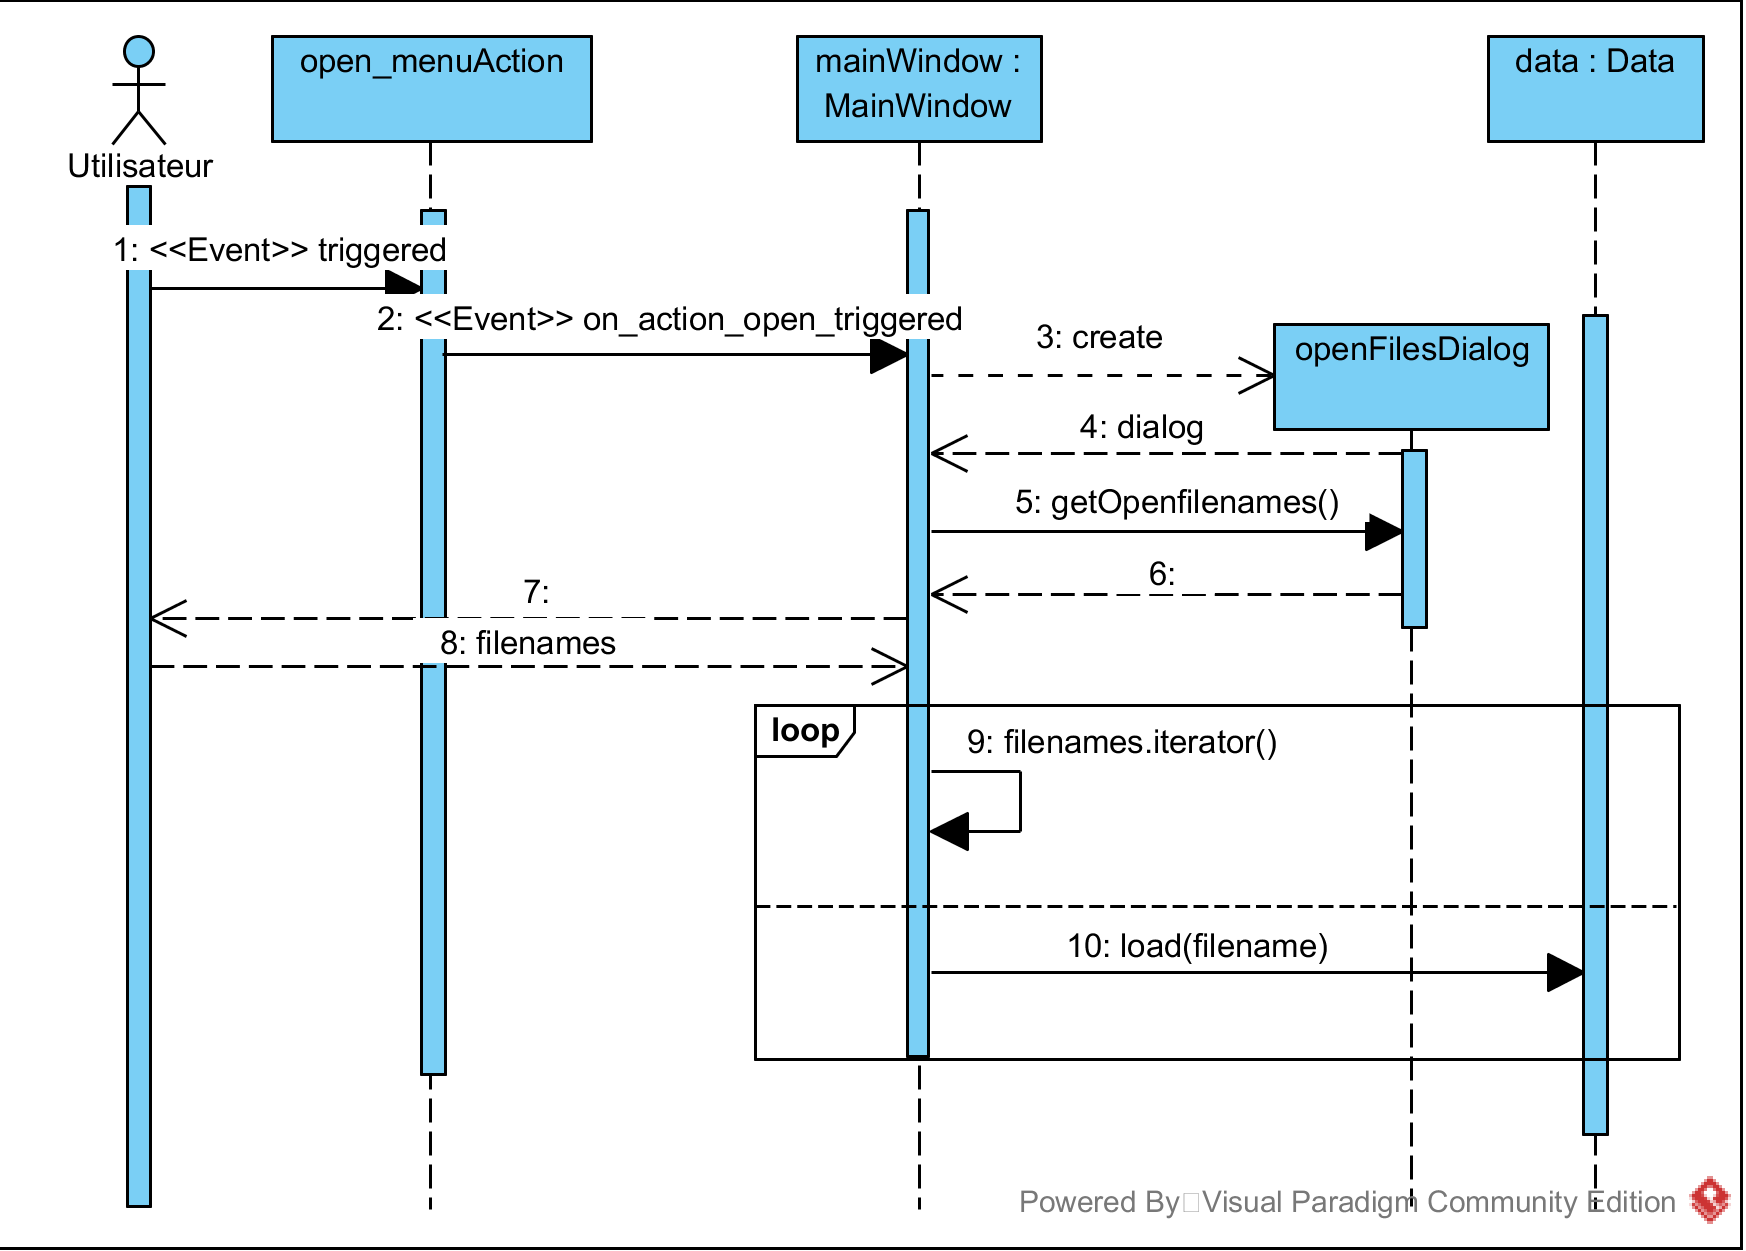
\includegraphics[scale=1]{dia_sequence_openFiles.png}
		\caption{Diagramme de séquence illustrant l’ouverture de fichiers données}
		\label{fig:seq_openFiles}
		\end{center}
		\end{figure}
			
		Lorsque le programme est lancé, aucune donnée n’est chargée, c’est à l’utilisateur de le faire en spécifiant les chemins des fichiers à ouvrir avec un explorateur de fichier classique. Il est possible de charger plusieurs fichiers à la fois, dans différents formats possibles (uniquement ceux supportés) (cf. Figure \ref{fig:seq_openFiles}).\\
	Une action de l’utilisateur (1) au niveau de l’interface graphique notifie le contrôleur de la requête (2). En conséquence, le contrôleur demandera auprès de l’utilisateur de spécifier les noms des fichiers et de les récupérer (3 à 8). Le contrôleur va ensuite itérer sur chacun des fichiers spécifiés pour les passer en paramètre de la méthode \textit{load} de classe \textit{Data} (9 à 10).
	
		\newpage
		\subsection{Fermeture de fichiers}
		\begin{figure}[!h]
		\begin{center}
		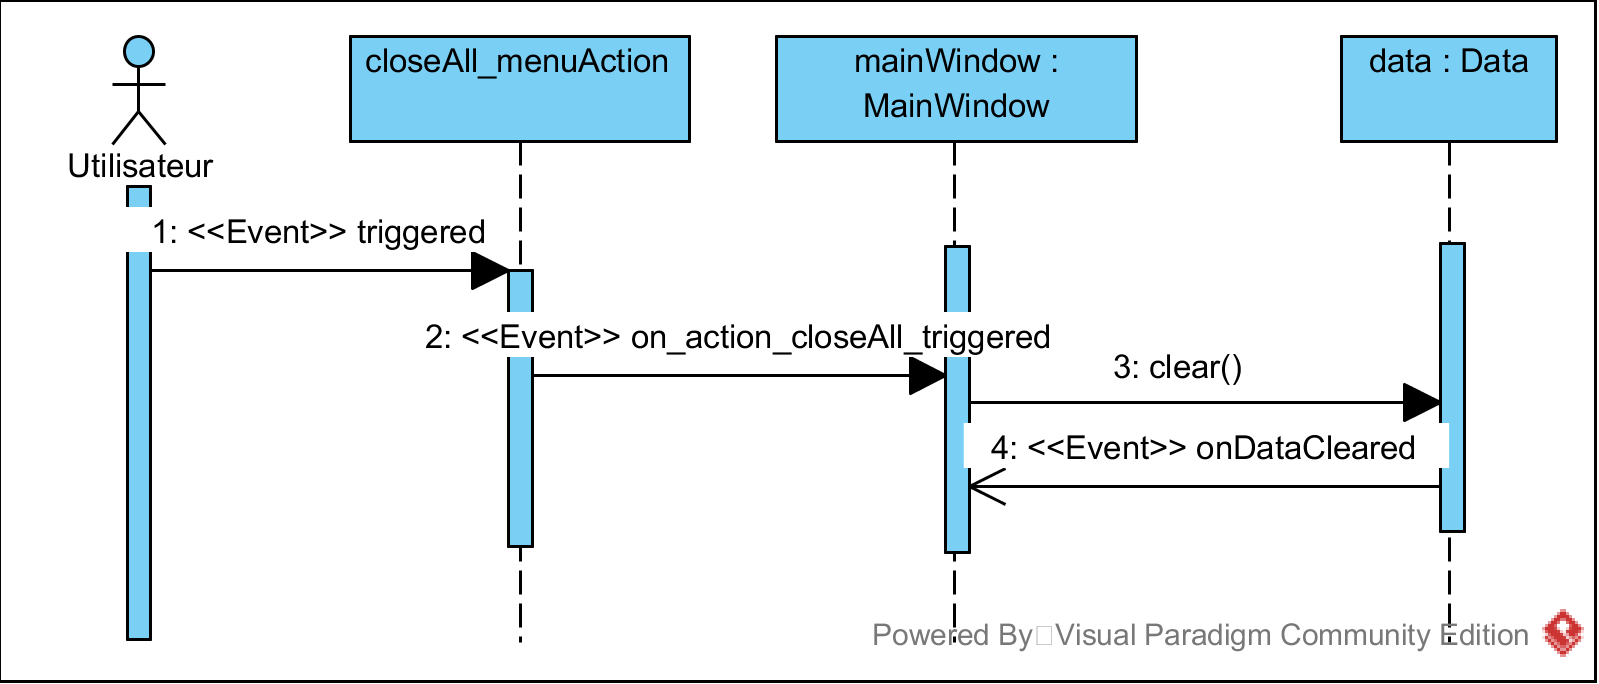
\includegraphics[scale=1]{dia_sequence_closeFiles.png}
		\caption{Diagramme de séquence illustrant la fermeture des fichiers ouverts}
		\label{fig:seq_closeFiles}
		\end{center}
		\end{figure}
			
		La séquence d’appel pour la fermeture des fichiers ouverts est analogue à celle pour l’ouverture (cf. Figure \ref{fig:seq_closeFiles}). L’action de l’utilisateur notifie le contrôleur de sa requête (1 à 2). En réponse, le contrôleur effectue un appel de la méthode \textit{clear} de la classe \textit{Data} (3).
			
			
		\subsection{Représentation des données (trajets et stations)}
		\begin{figure}[!h]
		\begin{center}
		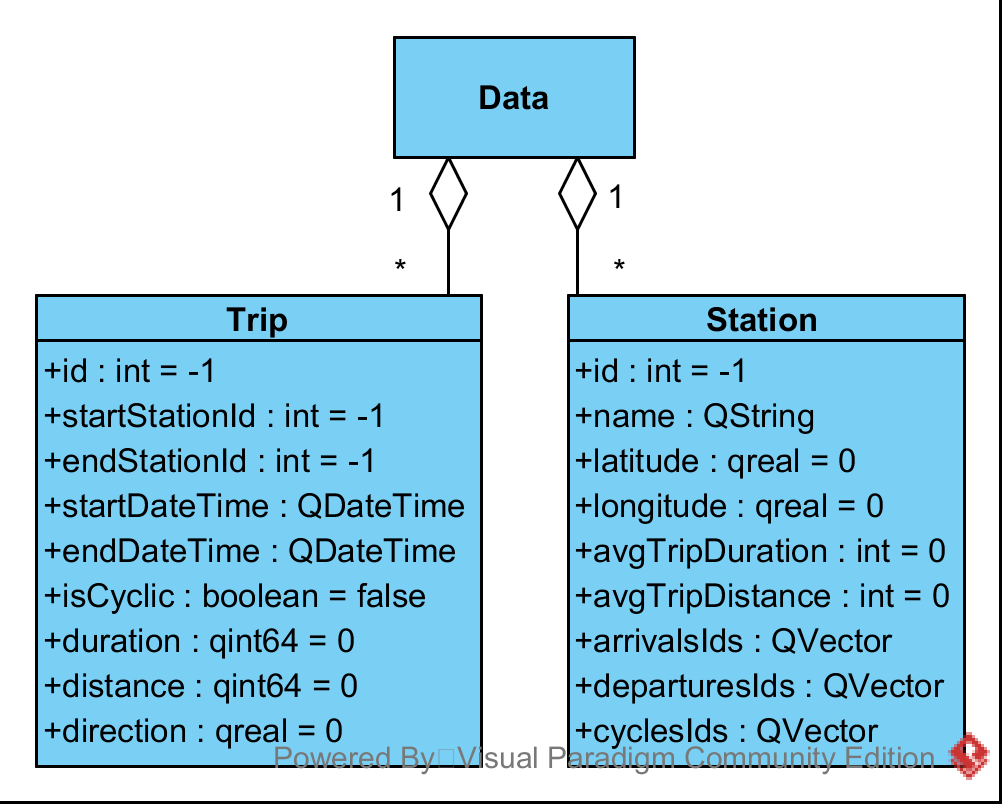
\includegraphics[scale=1]{dia_class_data.png}
		\caption{Représentation des données}
		\end{center}
		\end{figure}		
			
		Les données à manipuler sont représentés par des structures aux attributs publics,
		initialisés lors du parsing des fichiers. Ces entités sont passives, elles ne possèdent
		pas de méthodes qui produisent ou modifient d’autres objets. Ce sont
		donc des “classes-enregistrement” qui ne font que structurer la représentation des
		données.\\		
			
		\textbf{Trip}\\
		Cette structure contient les données nécessaires au filtrage et sélection des
		trajets :\\		
		\begin{itemize}
			\item[•]ses temps de départ et d’arrivée (comprend la date ainsi que l’heure)
			\item[•]sa durée (en secondes, codée par un entier sur 64 bits, initialisée à
			0 par défaut)
			\item[•]sa distance (en mètres, codée par un entier sur 64 bits, initialisée
			à 0 par défaut)
			\item[•]sa direction (ou azimut, en degrés, codée sur un réel, initialisée à
			0 par défaut)
			\item[•]un flag pour indiquer s’il est cyclique ou non (faux par défaut)\\
		\end{itemize}
			
		La distance et la direction sont codées sur des entiers 64 bits plutôt que 32 bits car on ne fait pas de supposition sur la durée ou distance maximale d’un trajet. Ils doivent être signés car on peut effectuer des opérations arithmétiques sur ces données. Malgré tout, il est important de fixer des limites (qui correspondent à celles du matériel).\\
			
		\textbf{Station}\\
		Cette structure contient les données nécessaires au filtrage et tri des stations :\\
		\begin{itemize}
			\item[•]son nom (sous forme de chaîne de caractères)
			\item[•]ses coordonnées géographiques (latitude et longitude) (en degrés,
			des réels initialisés à 0)
			\item[•]la distance moyenne (en mètres) d’un trajet (un entier, qui vaut 0 par défaut)
			l\item[•]a durée moyenne (en secondes) d’un trajet (un entier, qui vaut 0 par défaut)
		\end{itemize}
			
		\subsection{Association entre les stations et les trajets}
		Un trajet est obligatoirement associé à deux stations : celle d’arrivée et celle de départ.
	L’association ne se fait pas de manière classique avec des pointeurs mais avec des identifiants. Ces identifiants sont codés par des entiers. Ils sont initialisés par défaut à -1 pour indiquer qu’ils sont invalides. Les données valides sont initialisées lors du parsing des fichiers. L’identifiant d’une donnée est alors égale à sa position (son indice) dans le container qui le contient. Par exemple, le premier trajet parsé aura un identifiant égal à 0, puisque c’est le premier élément. C’est aussi pour cette raison que les identifiants sont codés sur des entiers 32 bits : ils correspondent à la taille du conteneur, qui est un entier 32 bits. On fixe ici, par la même occasion, les nombres maximaux de trajets et stations pouvant être chargés (qui est environ 2 milliards). Il faut savoir que pour environ 8000 trajets, on compte environ 360 stations différentes. Le nombre de stations est donc négligeable par rapport au nombre de trajets. Il faut également savoir qu’un fichier type pour une ville atteint environ 1 million de trajets. Là encore, il faudrait charger environ mille fichiers pour atteindre la limite d’un conteneur (avant que le programme ne crash).\\
	
	Cette manière d’associer les données a des avantages et des inconvénients.\\
			
		\textbf{Avantages}:
		\begin{itemize}
			\item[•] représentation simple, similaire à celle utilisée en base données.
			\item[•] évite l'utilisation des pointeurs, l’allocation avec l’opérateur \textit{new}, et donc les memory leaks (fuites de mémoire)
		\end{itemize}
			
		\textbf{Inconvénients}:
		\begin{itemize}
			\item[•] les opérations de filtrages, tris et sélection requièrent non pas les
			indices de ces données mais les données elles-mêmes. Il faut donc, à chacune de
			ces opérations, récupérer les données correspondantes, les traiter, et enfin
			les reconvertir en indices qui correspondent à ces données. Ces opérations
			de conversions indices vers données et vice-versa sont coûteuses en temps
			de calcul. C’est un point qui peut être résolu et qui est expliqué dans
			la section \ref{ameliorations} des améliorations possibles.
		\end{itemize}
			
		\subsection{Parsing des données}
		Les données sont parsées à partir de fichiers textes. C’est la classe \textit{Data} qui
		gère le parsing des données, en utilisant un \textit{DataFileReader}.
					
		\subsubsection{La classe “DataFileReader”}
	C’est une classe qui est utilisée localement par la classe \textit{Data} pour parser et charger les données. Elle hérite de la classe \textit{AbstractDataFileReader}, qui définit les prototypes des méthodes de parsing des données. \textit{DataFileReader} utilise en interne des parseurs spécialisés (qui héritent également de la classe abstraite) selon le type du fichier : elle utilisera :\\
	
		\begin{itemize}
			\item[•]un “CsvDataFileReader” pour parser un fichier CSV
			\item[•]un “XmlDataFileReader” pour parser un fichier XML
			\item[•]un “JsonDataFileReader” pour parser un fichier Json\\
		\end{itemize}
	
	
		\subsubsection{DataFileReadInfo}
		\begin{figure}[!h]
		\begin{center}
		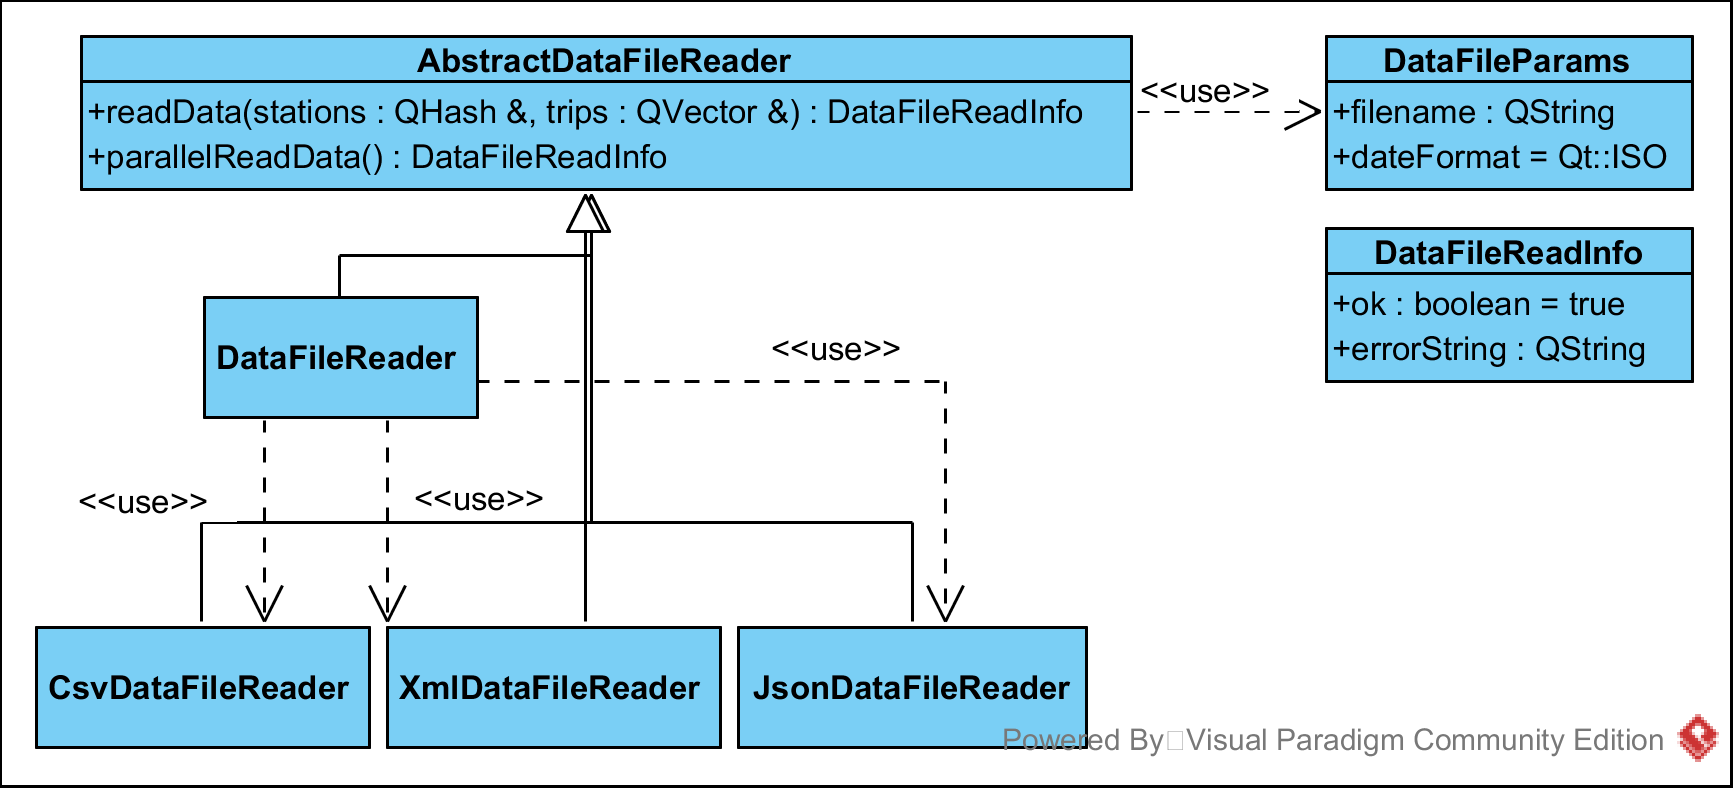
\includegraphics[scale=1]{dia_class_parsing.png}
		\caption{Hiérarchie des classes impliquées dans le parsing des données}
		\end{center}
		\end{figure}
			
		C’est le résultat retourné par une opération de parsing. Elle contient une chaîne de caractère, ainsi qu’un flag (mis à “vrai” si l’opération est un succès, “faux” sinon, auquel cas, la chaîne de caractère contient le message d’erreur).
	Ce résultat est transmis à la classe \textit{Data}.
			
		\subsubsection{La classe “Data”}
	Elle charge les données en utilisant un \textit{DataFileReader}, les stocke, permet un accès de celles-ci en lecture seule. Elle notifie également le contrôleur de ses actions réalisées en émettant des signaux (cf. Figure \ref{fig:dia_classe_modele}). Une donnée est indexée par son identifiant. Data permet également de savoir si elle a des données chargées avec le flag \textit{hasData}. Elle permet enfin de récupérer le nombre de trajets et stations avec les getter \textit{tripsCount} et \textit{StationsCount}.
	
		\begin{figure}[!h]
		\begin{center}
		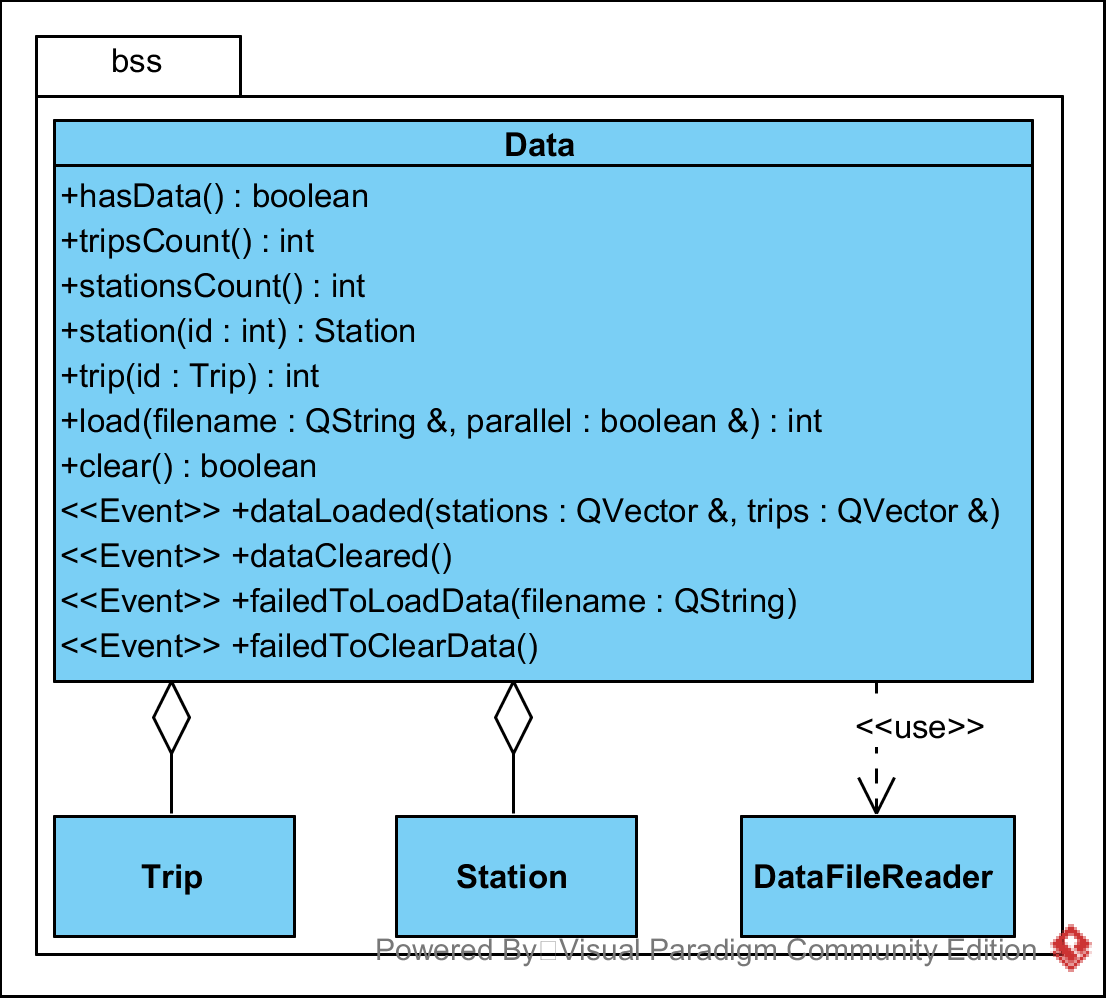
\includegraphics[scale=1]{dia_class_modele.png}
		\caption{Diagramme de classe des classes du modèle}
		\label{fig:dia_classe_modele}
		\end{center}
		\end{figure}
		
		\textit{Data} utilise un \textit{DataFileReader} pour parser les données, qui est créé lors d’un appel de la méthode \textit{load} de la classe \textit{Data} (cf. Figure \ref{fig:dia_seq_chargement_donnees}). C’est le contrôleur qui fait l’appel, en spécifiant un nom de fichier, récupéré au préalable auprès de l’utilisateur. \textit{Data} appelle ensuite la méthode \textit{readData} du \textit{DataFileReader}.\\
	
		Il est important de noter qu’il n’est pas indiqué sur la Figure \ref{fig:dia_classe_modele} le fait que cette méthode prend en paramètre et par référence un \textit{QHash} (table de hash) dont les clés sont des chaînes de caractères et les valeurs des stations, ainsi qu’un \textit{QVector} de trajet. Ce sont ces paramètres qui vont contenir les données. Les stations sont uniques par leurs noms, ce qui justifie le choix du type. Par la suite, la classe Data récupérera les stations en stockant dans un \textit{QVector} les valeurs de la table de hash. Il est également important de noter que les paramètres sont modifiés en ajout, c’est-à-dire que les données existantes ne sont pas effacées des paramètres. Enfin, il existe une variante de la méthode \textit{readData} nommée parallelReadData qui en plus des paramètres évoqués ci-dessus, prend en paramètres deux verrous (un pour le conteneur des stations, l’autre pour les trajets) et implémente un parsing en parallèle des données, avec des sections critiques. C’est l’association entre les trajets et les stations qui rend le parsing difficilement parallélisable, et qui force à passer en paramètre les données existantes (parser un nouveau fichier requiert de connaître les stations préalablement parsée, afin d’éviter les doublons et aussi de connaître le nombre de stations existantes car les identifiants des nouvelles en dépendent).\\
		
		\begin{figure}[!h]
		\begin{center}
		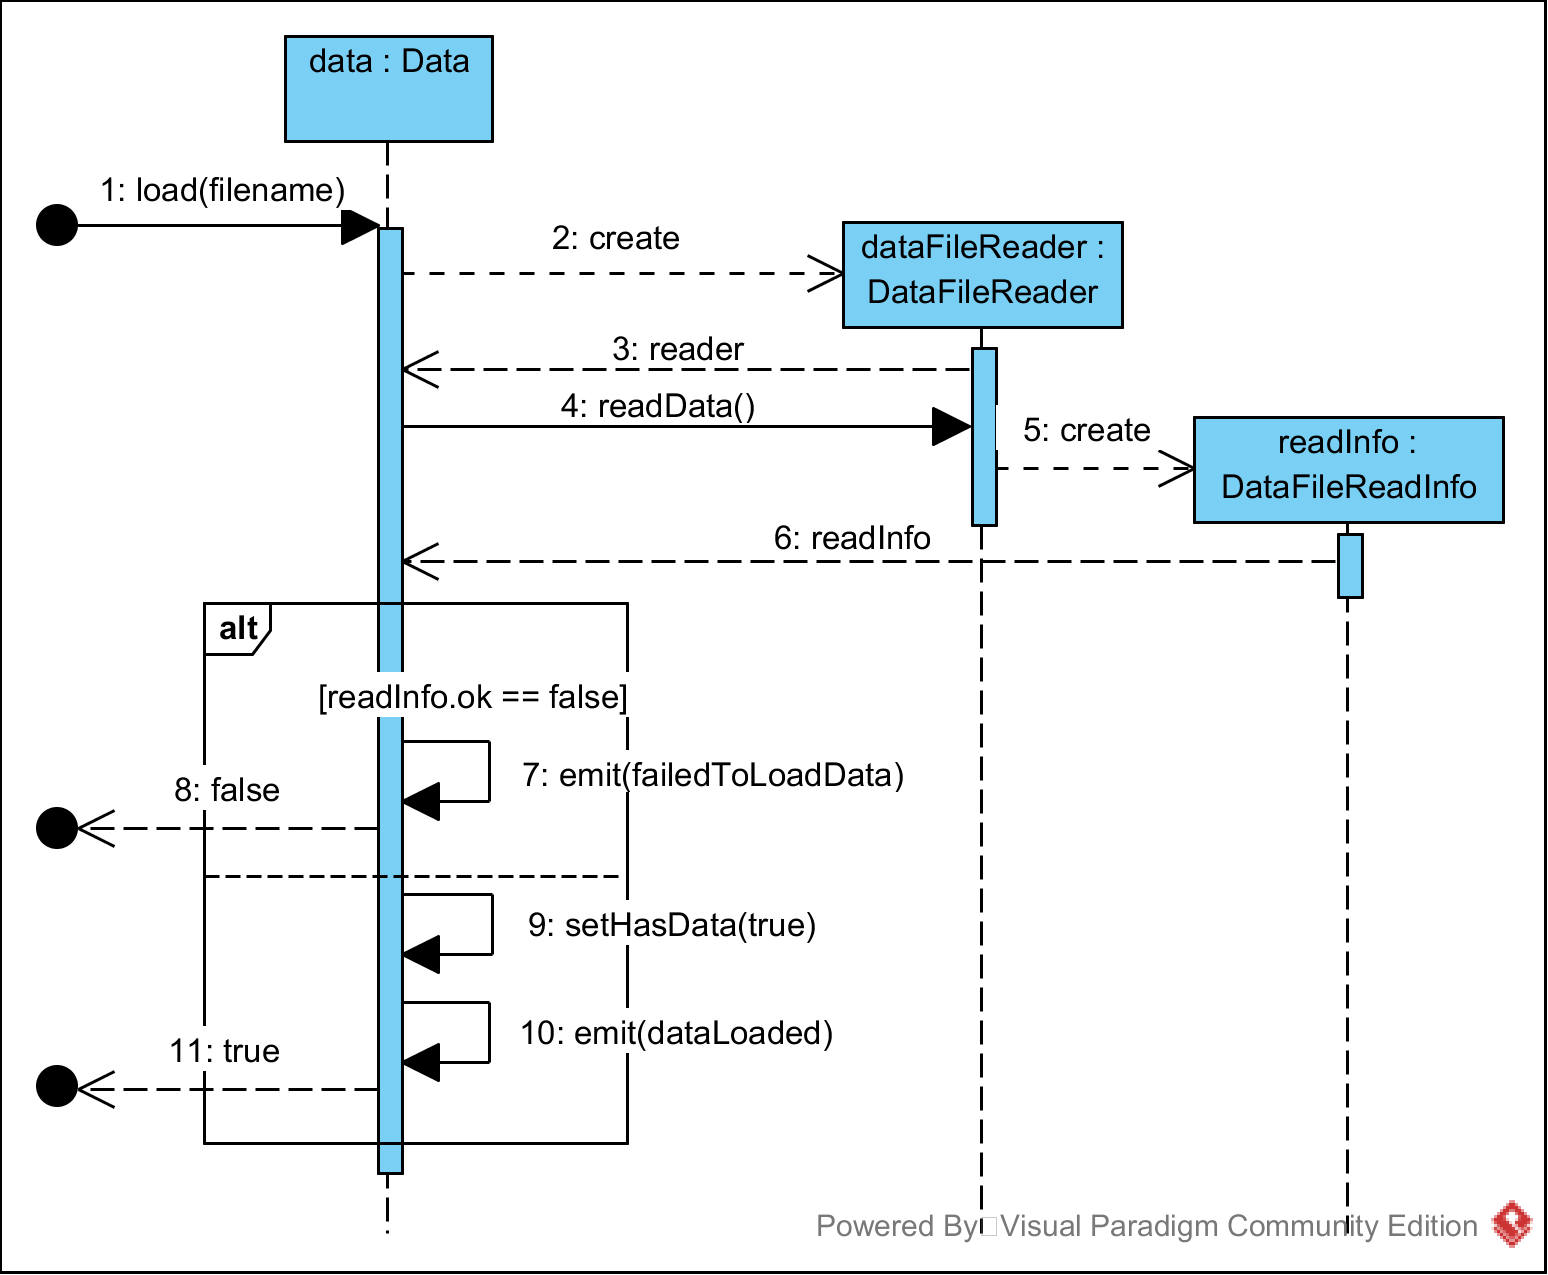
\includegraphics[scale=1]{dia_sequence_loadData.png}
		\caption{Diagramme de séquence illustrant le chargement des données}
		\label{fig:dia_seq_chargement_donnees}
		\end{center}
		\end{figure}
	
		L’appel à \textit{readData} retourne une structure \textit{DataReadInfo}. Si le parsing s’est déroulé sans erreur, son flag \textit{ok} vaut “vrai” et auquel cas l’appel de \textit{load} de la classe \textit{Data} renvoie “vrai”, après avoir émis le signal \textit{dataLoaded}. Le flag \textit{hasData} est mis à “vrai” pour indiquer que la classe \textit{Data} contient des données. Il est possible que le parsing se soit mal déroulé, par exemple si l’extension du fichier spécifié en paramètre n’est pas supporté pour le parsing, ou si le fichier est introuvable, invalide, ou autre. Dans ce cas, le flag \textit{ok} de la structure résultante vaut “faux”, et sa chaine de caractère \textit{errorString}contient le message d’erreur. Auquel cas, l’appel de \textit{load} de la classe \textit{Data} renvoie “faux”, après avoir émis le signal \textit{failedToLoadData}.
		
		\newpage
		\subsection{Courbes de Bézier}
		Les trajets sont dessinés par des courbes dans la \textit{mapglwidget}. Pour avoir de belles
		courbes, nous avons implémenté des courbes de Bézier. Elles sont faciles à implémenter et sont
		paramétrables.\\
		
		Les courbes de Bézier sont des courbes paramétriques qui sont définies par
		des points de contrôles.\\
		Dans notre cas, nous avons utilisé des courbes de Bézier de degrés 2 (quadratique). Ainsi,
		en passant 3 points en paramètre de notre fonction, on sera capable de générer une
		courbe (bien sûr, cela dépend du nombre de points que l'on génère, plus il y a de points,
		plus la courbe sera lisse).\\
		Pour ce faire, on prend un point \textit{P0} (le point de départ d'un trajet), un
		point \textit{P2} (le point d'arrivé du trajet) et un point \textit{P1} qui sera
		un point de contrôle que nous calculons.\\
		Pour calculer ce point, on prend la distance d'un trajet que l'on divise par 2. Ensuite,
		on calcule un point \textit{M} comme étant le milieu de ce segment. Pour finir, on cherche la
		position du point \textit{P1} de manière à ce que ce point passe par \textit{M} et que le
		segment $\overline{P1 M}$ soit perpendiculaire au segment $\overline{P0 P2}$ et
		de longueur $\left\lVert \frac{\overline{P0 P2}}{2}\right\rVert$. Bien entendu, cette
		dernière peut être différente, on peut très bien prendre le tiers $\overline{P0 P2}$ ou autre.
		Nous avons choisi la moitié, car cela semble visuellement à ce que nous cherchions. Prendre
		une distance plus grande rendrait les courbes trop bombées pour les longs trajets. \\
		
		Ainsi, avec nos 3 points et la formule suivante:
		
		\[
			{\mathbf  {B}}(t)=(1-t)^{{2}}{\mathbf  {P_{0}}}+2t(1-t){\mathbf  {P_{1}}}+t^{{2}}{\mathbf  {P_{2}}}{\mbox{ , }}t\in [0,1].
		\]
		
		on peut générer de nouveaux points (cf : code GLSL dans les annexes \ref{code_courbes_bezier}).
	
	\newpage
	\section{Stockage des données}
	Une fois les données chargées, elles sont stockées au sein de la classe \textit{Data}, dans des \textit{QVector}, classe générique qui joue le rôle de conteneur extensible similaire au \textit{std::vector} de la librairie standard. C'est le conteneur de premier choix, selon la documentation de Qt qui explique que son allocation contiguë de la mémoire permet un accès plus performant que les autres conteneurs.
	L’ajout se fait en passant en paramètre l’item à insérer à la méthode \textit{append}. Cette méthode est équivalente au \textit{pushback} du vecteur de la librairie standard (ajout en fin de liste, en incrémentant la taille). La méthode réserve spécifie une taille (passée en paramètre) préférentielle, qui est utile lorsque l’on connaît à l’avance la taille du conteneur.\\

	Ces données sont accessibles au contrôleur (pour permettre les opération de filtrages, tris et sélection) en lecture seule, afin d’éviter qu’il ne les errone par erreur.\\

\newpage
	\section{Nettoyage des données}
	Le nettoyage de données permet à l'utilisateur de décharger les données et ainsi nettoyer
	les éléments dessinés sur les différentes fenêtre d'affichage. Cela permet de charger 
	d'autres jeux de données sans tenir compte des données précédemment chargées.\\
	
	\begin{figure}[!h]
	\begin{center}
	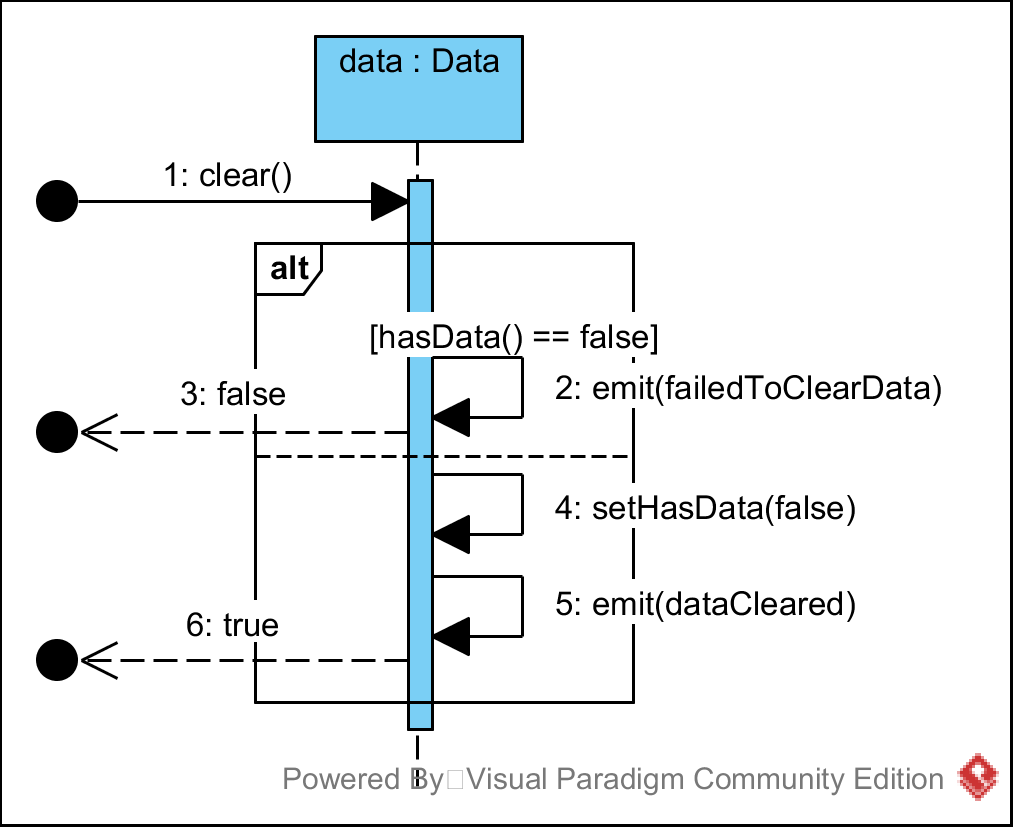
\includegraphics[scale=1]{dia_sequence_clear.png}
	\caption{ Diagramme de séquence du nettoyage des données}
	\label{fig:nettoyage}
	\end{center}
	\end{figure}
	
	Le nettoyage des données suit un schéma analogue à celui du chargement (cf. figure \ref{fig:nettoyage}). L’appel à la méthode \textit{clear} de la classe \textit{Data} teste le flag \textit{hasData} de cette même classe : s’il est négatif, la fonction retourne “faux”, après avoir émis le signal \textit{failedToClearData}. Si le test est positif, la fonction vide les conteneurs des données (non indiqué sur le schéma), positionne son flag \textit{hasData} à “faux” et retourne “vrai”, après avoir émis le signal \textit{dataCleared}.

\newpage
	\section{Traitement des données}
	On entend par traitement des données filtrage et sélection des trajets, ainsi que filtrage et tri des stations. Chaque traitement est effectué par un petit objet, paramétré par une structure de donnée.
	
	\begin{figure}[!h]
	\begin{center}
	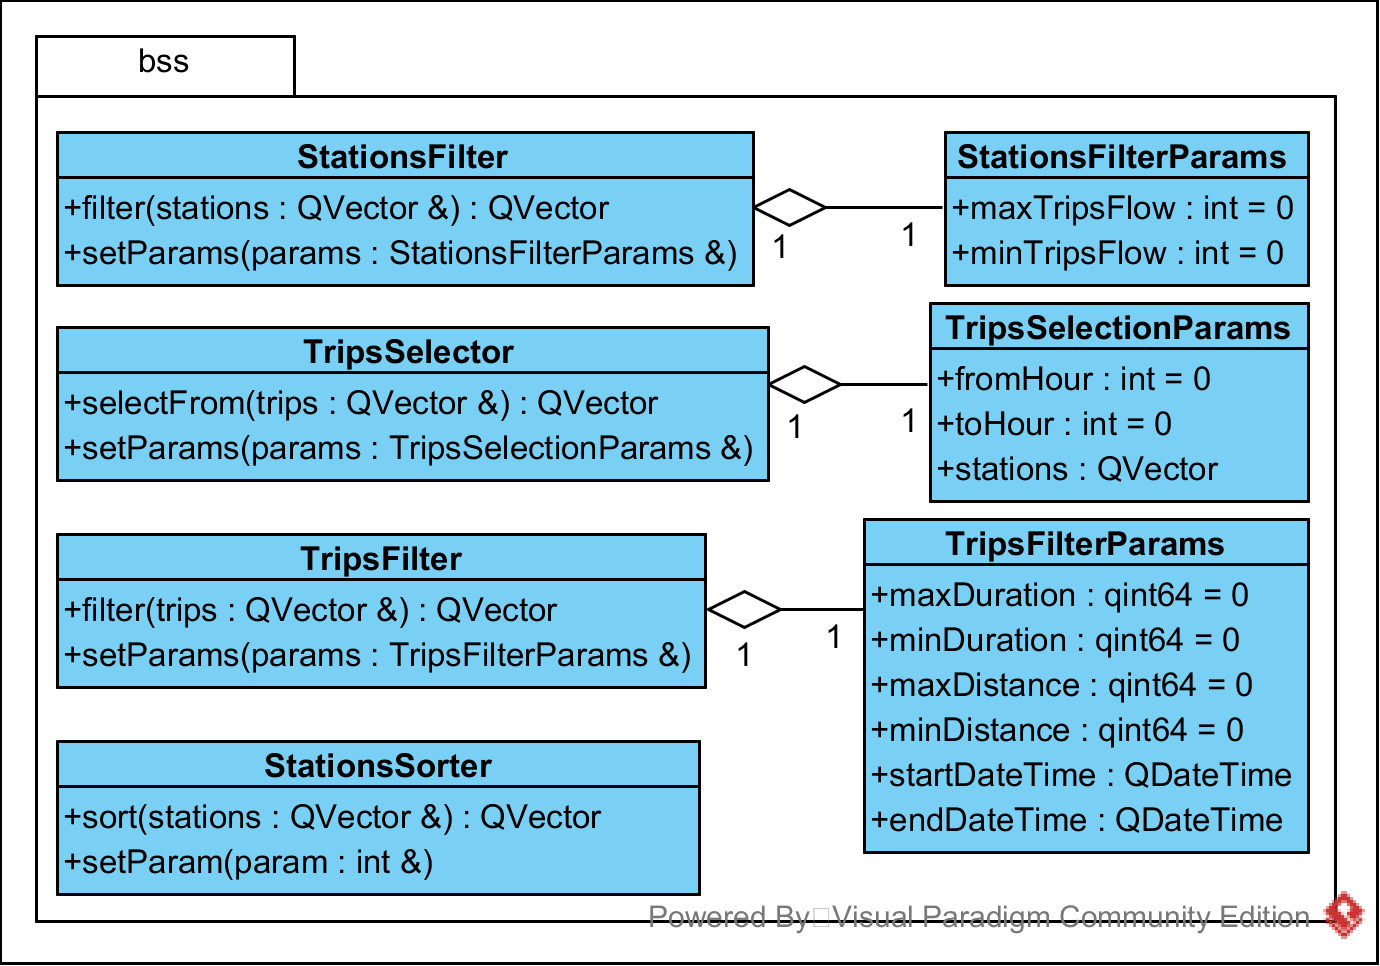
\includegraphics[scale=1]{dia_class_filtres.png}
	\caption{Diagramme de classe des classes impliquées dans le traitement des données}
	\end{center}
	\end{figure}
	
	\textbf{Filtrage des stations} : c’est l’objet \textit{StationsFilter} qui en est chargé, avec l’appel de \textit{filter} qui prend en paramètre les stations à filtrer, et retourne les stations filtrées. Cet objet est paramétré par une structure \textit{StationsFilterParams}, qui contient un intervalle d’entiers (initialisés à 0), afin de filtrer sur le flux de trajets des stations.\\

	\textbf{Sélection des trajets} : c’est l’objet \textit{TripsSelector} qui en est chargé, avec l’appel de \textit{selectFrom} qui prend en paramètre l’ensemble des trajets à partir desquels il faut appliquer la sélection. Il retourne les trajets répondant aux critères de sélection. Cet objet est paramétré par une structure \textit{TripsSelectionParams}, qui contient un intervalle d’entiers (initialisés à 0), afin de filtrer sur l’intervalle de temps du trajet, ainsi qu’une liste des identifiants des stations auxquelles les trajets sélectionnés doivent être associés.\\

	\textbf{Filtrage des trajets} : c’est l’objet \textit{TripsFilter} qui en est chargé, avec l’appel de filter, qui prend en paramètre l’ensemble des trajets à partir desquels il faut appliquer le filtre. Il retourne les trajets filtrés. Cet objet est paramétré par une structure \textit{TripsFilterParams}, qui contient un intervalle d’entiers (initialisés à 0), afin de filtrer sur l’intervalle de temps du trajet, ainsi qu’une liste des identifiants de stations.\\

	\textbf{Tri des stations} : c’est l’objet \textit{StationsSorter} qui en est chargé, avec l’appel de sort, qui prend en paramètre l’ensemble des stations à trier. Il retourne les stations triées. Cet objet est paramétré par un type énuméré qui code une propriété de station. Les valeurs possibles du paramètre sont : \textit{DISTANCE}, \textit{DURATION}, \textit{ARRIVALS}, \textit{DEPARTURES}, et \textit{CYCLES}. Le tri se fait par ordre décroissant selon la propriété (par exemple, si on filtre sur le nombre de départs, une station associée à deux départs est placée avant une stations associée à un seul départ).\\
	
	\begin{figure}[!h]
	\begin{center}
	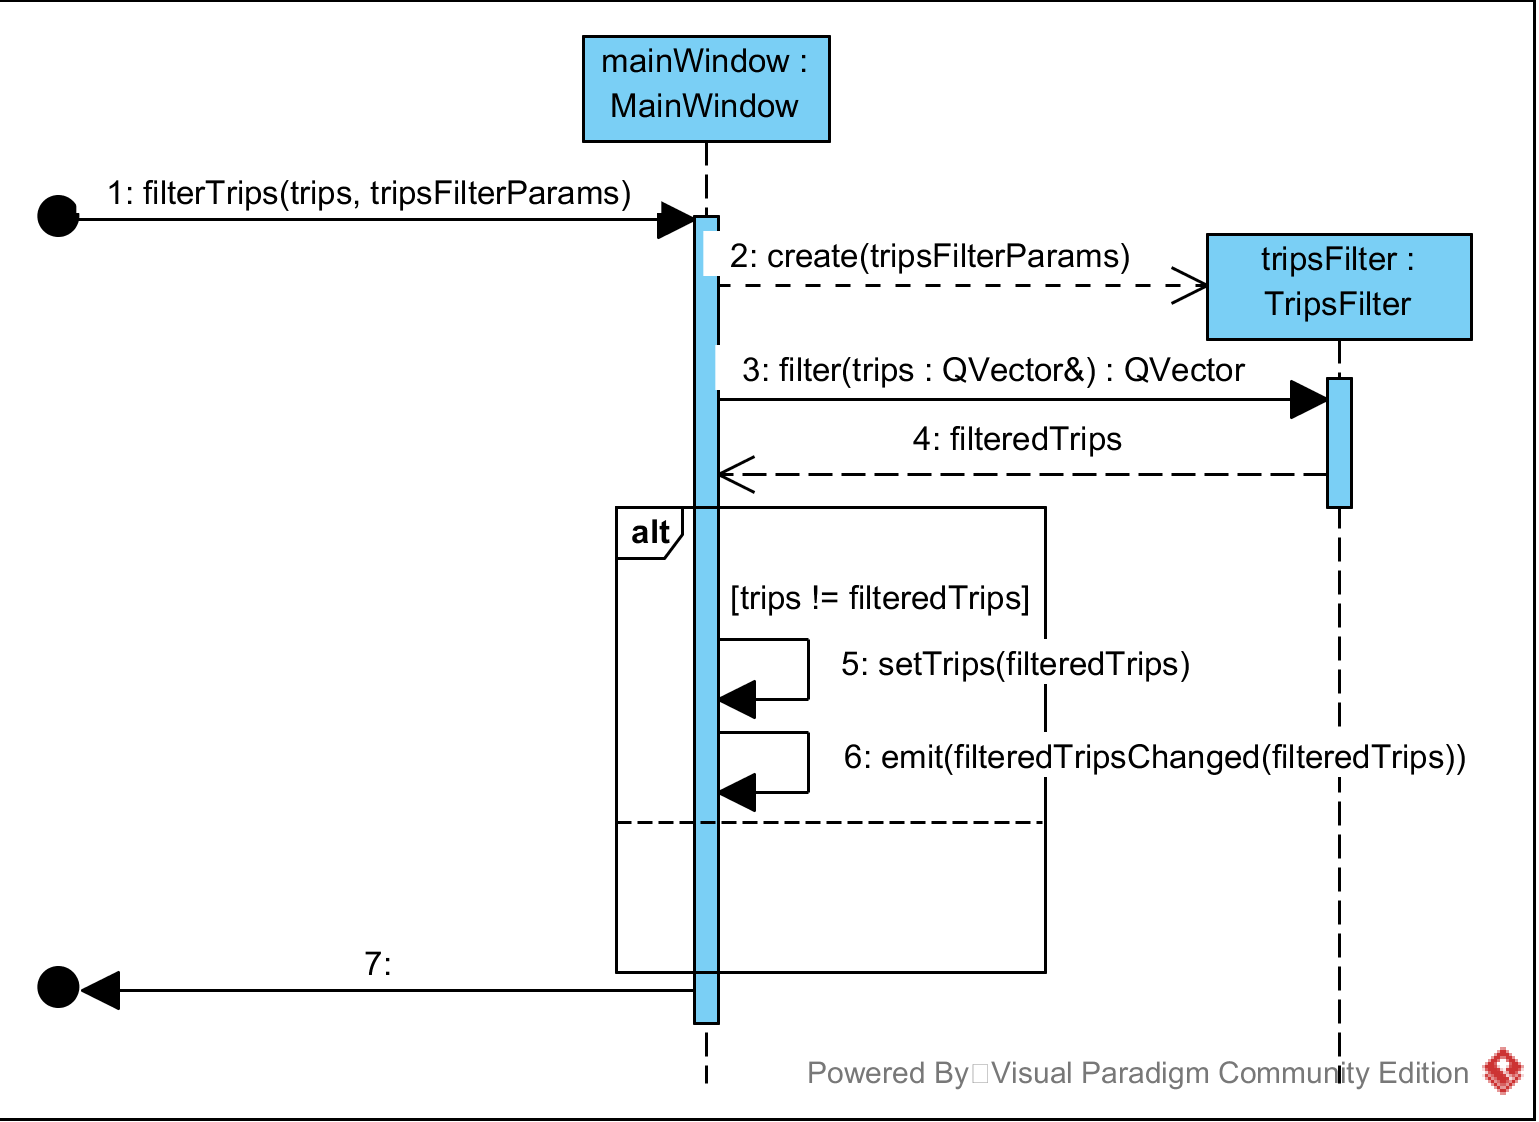
\includegraphics[scale=1]{dia_sequence_filterTrips.png}
	\caption{Diagramme de séquence de l’opération de filtrage des trajets}
	\label{fig:filterTrips}
	\end{center}
	\end{figure}

	Le diagramme de la figure \ref{fig:filterTrips} illustre la séquence d’appel depuis le contrôleur lors d’un filtrage de trajets. L’appel à \textit{filterTrips} survient lorsque l’utilisateur souhaite filtrer les trajets. Il prend en paramètre les trajets à filtrer (le contrôleur entretient non pas les données mais les identifiants de ces données, il aura donc fallu au préalable avoir récupéré les trajets correspondant à ces identifiants) ainsi que les paramètres de filtrage. Il s’ensuit l’utilisation du \textit{TripsFilter}. Après filtrage, si les trajets filtrés sont différents de ceux dont le contrôleur entretient, il met à jour ses trajets, et émet un signal.\\
	
	\begin{figure}[!h]
	\begin{center}
	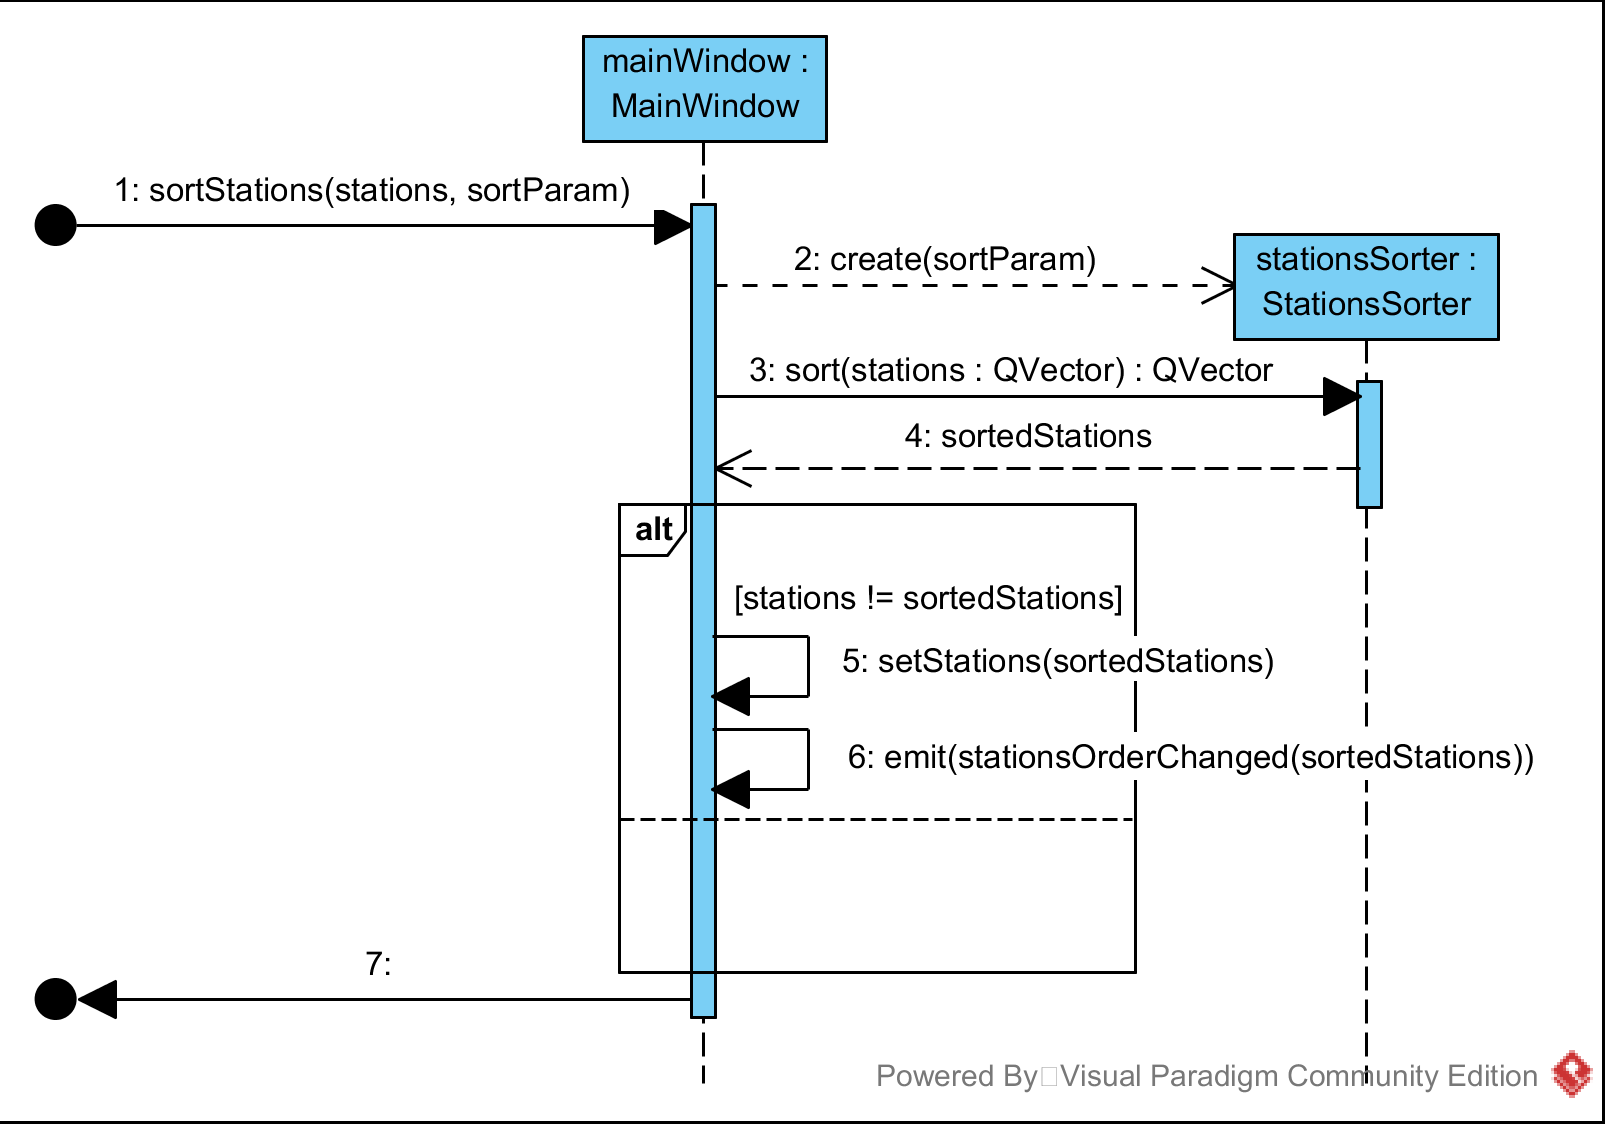
\includegraphics[scale=1]{dia_sequence_sortStations.png}
	\caption{Diagramme de séquence de l’opération de tri des stations}
	\label{fig:sortStations}
	\end{center}
	\end{figure}
	
	Le diagramme de la figure \ref{fig:sortStations} illustre la séquence d’appel depuis le contrôleur lors d’un tri des stations. Le schéma d’appel est sensiblement analogue à celui du filtrage des trajets expliqué plus haut. L’appel à \textit{sortStations} survient lorsque l’utilisateur souhaite trier les trajets. Il prend en paramètre les stations à trier ainsi que les paramètres de filtrage. Il s’ensuit l’utilisation du \textit{StationsSorter}. Après le tri, si les stations triées sont différentes de ceux dont le contrôleur entretient, il met à jour ses stations, et émet un signal.\\
	
	Il est important de noter que ces opérations sont lourdes, particulièrement celles concernant les trajets, puisque leur quantité pour une utilisation standard est importante (plusieurs centaines de milliers de trajets). C’est pourquoi ces opérations sont effectuées dans un autre thread que celui de l’interface graphique, ce qui explique le fait que le contrôleur émet des signaux à lui-même. Les signaux émis proviennent du thread en tâche de fond et sont reçus par le thread de l’interface graphique dès lors que la tâche lourde est terminée. Une seule tâche lourde peut-être exécutée à la fois. Une tâche devra attendre son tour avant d’être exécutée, si le thread en background est occupé. Si cela survient, le thread de l’interface graphique est bloqué (jusqu’à ce que la tâche qui attend son tour soit exécutée par le thread en background).\\
		
	\newpage
	\section{Classes de rendu graphique}
	
	\begin{figure}[!h]
	\begin{center}
	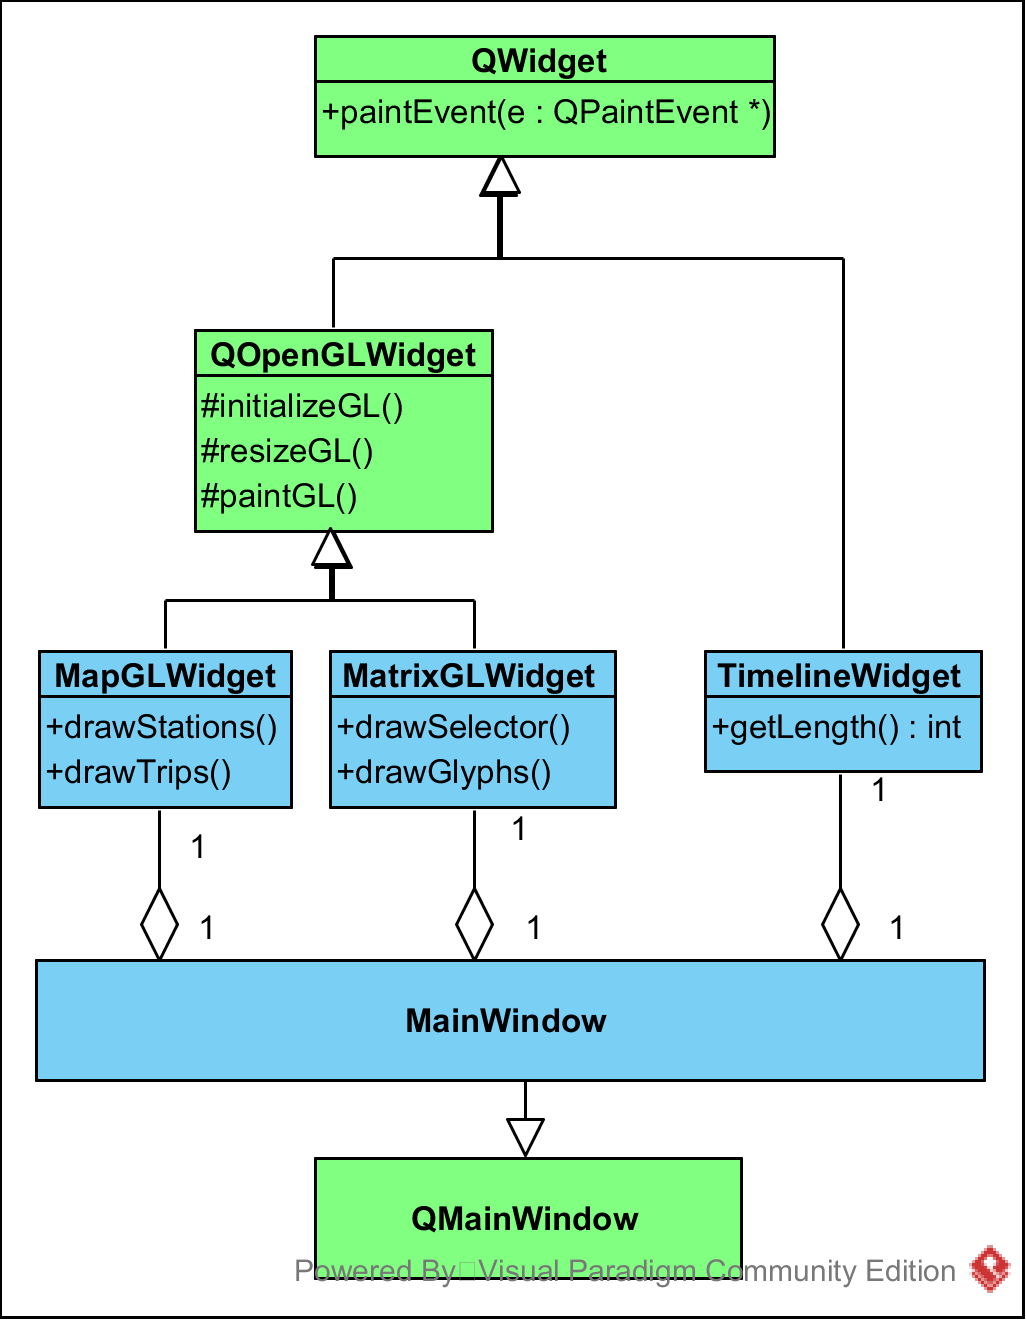
\includegraphics[scale=1]{dia_class_rendering.png}
	\caption{Diagramme de classe des vues}
	\label{fig:renduGraphique}
	\end{center}
	\end{figure}
	
	Les trois principales classes du rendu des trajets et des stations sont \textit{MapGLWidget}, \textit{MatrixGLWidget} et \textit{TimelineWidget}. Les deux premières sont des spécialisations de la classe \textit{QOpenGLWidget} qu’offre Qt. Elles permettent l’affichage des stations et des trajets. La troisième, c’est un \textit{QWidget}, dont le rôle est d’afficher une ligne de temps au
dessus de la \textit{MatrixGLWidget}.
	
		\subsection{Classe TimelineWidget}
		Pour réaliser l’affichage d’une ligne de temps à intervalle d’une heure, nous avons utilisé un \textit{QWidget} dont la fonction \textit{paintEvent} a été réimplémenté. La manière de réaliser cela est assez simple, nous avons utilisé un \textit{QPainter} pour tracer les lignes. Une longue ligne horizontale représente la ligne temps sur laquelle les heures sont définies, et les petits traits verticaux à chaque fois que l’on veut y faire afficher une heure.\\
Dans notre cas, nous avons utilisé vingt-quatre heure, mais ce nombre est paramétrable dans un fichier. De plus, la largeur des intervalles est re-calculée à  chaque fois que le widget est redimensionné
(cf Figure : \ref{fig:timeline_widget_1} et \ref{fig:timeline_widget_2}).


\clearpage
		\begin{figure}[!h]
		\begin{center}
		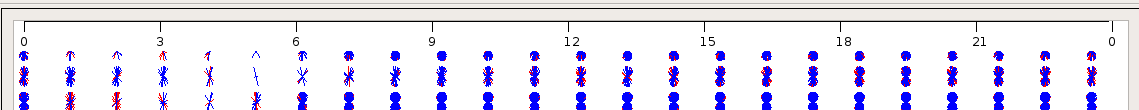
\includegraphics[scale=.4]{timeline_widget_1.png}
		\caption{Impression écran de la timelinewidget en plein écran (1920x1080)}
		\label{fig:timeline_widget_1}
		\end{center}
		\end{figure}
		
		\begin{figure}[!h]
		\begin{center}
		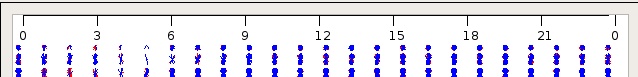
\includegraphics[scale=.4]{timeline_widget_2.png}
		\caption{Impression écran de la timelinewidget avec la fenêtre réduite}
		\label{fig:timeline_widget_2}
		\end{center}
		\end{figure}
		
		Les deux images ci-dessus (Figure : \ref{fig:timeline_widget_1} et \ref{fig:timeline_widget_2})
		sont affichées à la même échelle.
	
		
		\subsection{Classe MapGLWidget}
		Elle permet d’afficher les trajets ainsi que les stations en utilisant les fonctions d’OpenGL. Lorsque les données sont chargées dans la mémoire, le contrôleur (\textit{MainWindow}) fait appel à la fonction \textit{loadTripsData} et \textit{loadStationsData} afin d’envoyer les positions des stations et des trajets à la carte graphique via les objets \textit{StationRenderer} et \textit{TripsRenderer}. (cf : Figure \ref{fig:dia_class_renderer} plus bas) Ces objets possèdent une fonction \textit{sendData} qui prend en paramètre
		un tableau contenant les positions des trajets et stations. Cette fait appel à la fonction
		\textit{glBufferData}, une fonction OpenGL qui envoie les données à la carte graphique.\\

		Une fois les données chargées, le contrôleur va aussi appelé une fonction de centrage afin que l’utilisateur ai une vue sur l’intégralité des éléments dessinés avec un zoom adapté.
Pour calculer le centrage, on parcourt tous les points à dessiner en cherchant une boîte englobante de ces points. L’étape suivante consiste à trouver le centre de cette boîte, de sorte que, cx et cy, la position du centre de la boîte.\\

	Avec le milieu de la boîte englobante, on peut indiquer la translation en utilisant une variable
	\textit{uniform} à laquelle le shader calculera la position des vertices. Mais il faut aussi calculer la valeur du zoom pour que l’utilisateur puisse voir tous les éléments correctement.\\
	
	Les variables \textit{uniform}, sont des variables globales propres aux shaders. On les utilises
	pour envoyer des données de la mémoire physique aussi appelée RAM, vers la mémoire de la carte
	graphique.\\
	
	Les shaders sont des programmes, proches du langage C, qui sont exécutés par la carte graphique. Il
	en existe de différents types, chacun ont une fonction propre.\\

	Pour calculer ce zoom, il faut prendre la plus grande valeur entre la hauteur et la largeur de la boîte englobante, puis diviser deux par cette valeur maximale.\\

	zoom = 2.f / max(hauteur, largeur)\\

	Le 2 vient du fait que les coordonnées OpenGL vont de -1 à 1, donc la distance vaut 2.

	Ainsi, nous avons le zoom et la translation. Une fois envoyés au shaders, nous aurons un affichage correcte et approprié.\\

	Cette classe gère les événement de la souris comme l’utilisation de la molette pour zoomer ou dé-zoomer mais aussi lorsque l’utilisateur presse et relâche les boutons de sa souris pour effectuer des translation de la carte.
		
		\subsection{Classe MatrixGLWidget}		
		Cette classe a pour rôle d’afficher les glyphes pour chaque stations et pour chaque heures. De plus, elle doit permettre d’interagir avec la matrice de chronologie des trajets, comme défiler en
		haut et en bas avec la souris, ainsi que pouvoir sélectionner un ensemble de glyphes.\\

		L'implémentation du défilement est assez simple, puisqu'elle consiste à récupérer la valeur
		du défilement grâce à l'instance de la classe \textit{QWheelEvent} et envoyer au shader cette valeur pour l’affichage.\\

		Au moment de la sélection des glyphes, il faut récupérer l'événement de la souris pour connaître sa position au moment du click et une autre position lors du relâchement de la souris. Ainsi, cela peut former un rectangle que l’on se contente d’afficher. Cela est fait grâce à l’objet \textit{SelectorRenderer} (cf Figure \ref{fig:dia_class_renderer} plus bas). Avec les coordonnées du rectangle, on peut aussi savoir quels glyphes sont à l'intérieur du rectangle. Il suffira ensuite de récupérer les indices des stations et l’intervalle des heures pour émettre un signal est dessiner sur la carte les trajets sélectionnés\\

		Le rendu des glyphes en eux-même s’est avéré assez complexe et long à implémenter, puisque pour chaque glyphes, il faut dessiner une multitude de lignes avec un certain angle de rotation pour chacune de ces lignes. Pour chaque trajets, son azimut (de 0 à 360 degrés) est calculée. Cette direction permet de définir l'orientation de chaque segments dessinés dans la \textit{timelinematrix}.
		
\clearpage
		\subsection{Classes Renderer}
		
		\begin{figure}[!h]
		\begin{center}
		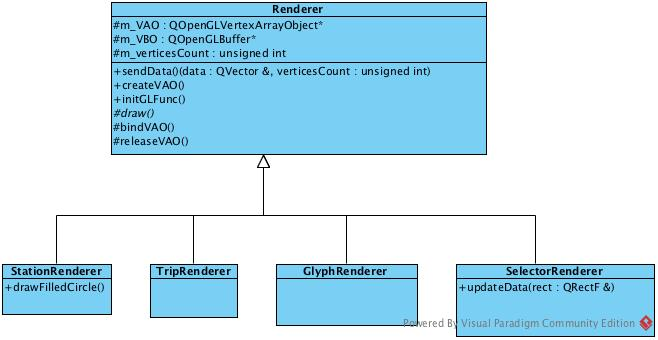
\includegraphics[scale=.7]{dia_class_renderer.png}
		\caption{Diagramme de classe de rendu graphique}
		\label{fig:dia_class_renderer}
		\end{center}
		\end{figure}		
		
		Le \textit{Renderer} est une classe abstraite dont chaque objet de rendu en hérite. Elle possède
		un \textit{VertexArrayObject} (VAO) et un \textit{VertexBufferObject} (VBO), ainsi que le nombre vertices à afficher.\\
		
		Les VBO peuvent être vus comme des tableaux peuvent contenir des positions ou des indices par exemples, dans notre cas ils stockent des positions.\\

		Les VAO, permettent d’optimiser le temps d’affichage (très légèrement) en encapsulant les données qui lui sont associées. Il garde une référence sur les VBO.\\
		
		La méthode \textit{draw} est virtuelle pure, c’est à dire que la classe qui hérite de \textit{Renderer} doit obligatoirement implementer celle-ci.\\

		Elle contient une fonction, \textit{sendData} pour envoyer les données à la carte graphique avec \textit{glBufferData}. La fonction \textit{createVAO} créé et active le VAO et VBO.\\		
		
		Les classes filles sont relativement simples:\\
		
		\textbf{StationRenderer}\\
		Cette classe hérite de Renderer, elle dessine des stations qui sont représentées par des points. Une fonction drawFilledCircle a été implémentée mais n’est pas utilisée et n’a pas été testée.\\
		
		\textbf{TripsRenderer}\\
		Cette classe hérite de Renderer, elle dessine des trajets par des lignes. \\

		\textbf{GlyphRenderer}\\
		Cette classe hérite de Renderer, elle dessine des glyphes par des lignes. \\
		
		\textbf{SelectorRenderer}\\
		Cette classe hérite de Renderer, elle dessine un rectangle coloré par deux triangles.
		
\newpage
\part{Outils}
	\section{Développement}
		\subsection{Installation de Qt}
		Pour installer Qt, nous avons simplement téléchargé les binaires disponibles de Qt 5.8
		sur le site :  \url{https://www.qt.io} \\
		
		Nous avons choisi Qt 5.8.0 pour Linux 64 bit.\\
		Une fois téléchargé, nous avons ouvert un terminal pour lancer le fichier \textit{\textbf{.run}} téléchargé.\\
		Enfin, nous avons suivi les étapes d'installation jusqu'à ce que l'installation se termine.
		
		\subsection{Installation de gcc}
		Pour installer \textit{gcc}, nous avons utilisé la commande suivante, qui permet de récupérer les paquets :
		\begin{verbatim}
		sudo apt-get install build-essential
		\end{verbatim}
		Cela nous a installé la version 4.9.2 de \textit{gcc}.
		

\newpage
\part{Les tests}
	\section{Les tests de performances} \label{tests_performances}
		\subsection{Conditions de tests}
		Les tests ont été réalisés sur un système d’exploitation Linux Debian 8.7 avec
		un noyau de version 3.16.0-4-amd64. \\ \\
		Spécifications de la machine: \\
		
		\begin{center}
			\begin{tabular}{| l | c |}
			\hline
			\textbf{Composants} & \textbf{Model} \\ \hline
			Processeur & Intel I5 2500k \\ \hline
			Carte Graphique & NVIDIA GTX 970 4Go \\ \hline
			Mémoire vive & 12 Go \\ \hline
			Disque dur & à 7200 trs/min \\ \hline
		    \end{tabular}
	    \end{center}
	    
	    Outils de développement: \\
	    \begin{center}
			\begin{tabular}{| l | c |}
			\hline
			\textbf{Outils} & \textbf{Version} \\ \hline
			gcc & 4.9.2 \\ \hline
			Qt & 5.8 \\ \hline
			Flags de compilation & C++14\\ \hline
		    \end{tabular}
	    \end{center}
	    
	    Le fichier utilisé pour tester les temps de chargement est disponible à ce lien:\\
		\url{https://s3.amazonaws.com/tripdata/201310-citibike-tripdata.zip}\\
		
		Le fichier contient 843 416 trajets et 329 stations. \\
		
		Chacun des tests ont été réalisés plusieurs fois (20 fois), ce
		sont les valeurs montrant les meilleurs performances qui ont été
		sélectionnées (Si un test montre 20 images par secondes et un second en montre
		10, c'est celui à 20 image par secondes qui sera sélectionné).
	    
		\subsection{Chargement des fichiers en mémoire}		
		\begin{center}
			\begin{tabular}{| l | c |}
			\hline
			\textbf{Méthode} & \textbf{temps (en millisecondes)} \\ \hline
			Séquentiel & 21 214 \\ \hline
			Parallèle & à tester \\ \hline
		    \end{tabular}
	    \end{center}
		
		\subsection{Affichage des trajets et des stations}
		\begin{center}
			\begin{tabular}{| l | c |}
			\hline
			\textbf{Méthode} & \textbf{temps (en millisecondes)} \\ \hline
			QPainter & 1396 \\ \hline
			OpenGL & 10.636 \\ \hline
		    \end{tabular}
	    \end{center}
	    
	    Le nombre de points généré ici est de 20 pour les courbes de Bézier.\\
	    	    
	    \subsection{Courbes de Bézier}
		Les courbes de Bézier sont évaluées dans les Geometry shaders. Les Geometry shaders
		permettent de modifiés les primitives tel que des lignes, les points ou les triangles
		en générant des nouveaux vertices. Nous avons fait le choix d'implementer cette 
		fonctionnalité dans un shader (cela aurait très bien pu être fait par le processeur)
		car théoriquement cela devrait être plus performant. En effet, la carte graphique
		traite les vertices de manière parallèle. Nous n'avons pas fait des tests
		comparatifs par manque de temps.\\
	    
		\begin{center}
			\begin{tabular}{| c | c |}
			\hline
			\textbf{Nombre de points générés} & \textbf{temps (en millisecondes)}\\ \hline
			5  &  8.771 \\ \hline
			10 &  5.586 \\ \hline
			15 &  8.773 \\ \hline
			20 &  15.874 \\ \hline
			25 &  10.636 \\ \hline
			30 &  12.5 \\ \hline
			50 &  21.939\\ \hline
			100 &  37.039 \\ \hline
		    \end{tabular}
	    \end{center}
	    
	    Un ensemble d'impressions écran se trouve dans les annexes (cf section \ref{}) afin
	    de pouvoir comparer le nombres de points générés. Selon nous, 20 points semble un bon être
	    un bon compromis.\\
	    
		\subsection{Affichage des glyphes}
		Dans la mesure où le temps d'affichage des trajets et des stations avec des \textit{QPainter}
		était déraisonnable, nous n'avons pas pris le temps coder l'affiche de glyphes. Cela serait 
		une perte de temps et les performances serait clairement inacceptable.
		
		\begin{center}
			\begin{tabular}{| l | c |}
			\hline
			\textbf{Méthode} & \textbf{temps (en millisecondes)} \\ \hline
			QPainter & Non testé\\ \hline
			OpenGL & 15.625 \\ \hline
		    \end{tabular}
	    \end{center}
		
	\newpage
	\section{Tests unitaires}
	Ils ont été effectués avec Bandit, comme conseillé par le client.
	Bandit est un framework C++11 de test unitaires, sous licence MIT. Il est disponible sur GitHub. 		Il faut aussi savoir qu’il est dépendant d’un autre framework : Snowhouse.\\

	Pour le faire fonctionner, il faut placer le dossier Bandit au même niveau que les fichiers d’en-tête du projet à tester.

	\url{http://banditcpp.org/}
	
		\subsection{Classe StationFilter}
		Pour tester la classe, on peut commencer par définir son comportement au sein de l’application.\\

		Lors de sa construction), elle reçoit en paramètre \textit{StationsFilterParams}, qui permet de régler les bornes. La fonction \textit{filter} reçoit un \textit{QVector} de stations pour lesquelles elle filtre l’attribut \textit{tripsFlow} en fonction des paramètres que nous avons préalablement réglé. Elle renvoie ensuite un \textit{QVector} des stations après application du filtre. Ces paramètres nous permettent de régler un minimum et un maximum. Pour tester cette fonction, nous avons testé si les bornes étaient bien réglées. Pour cela nous avons créé des stations, pour lesquelles nous initialisons la variable \textit{tripsFlow}.\\

		\textbf{TRIPS FLOW MIN} :\\
		Pour tester la borne minimum de cette propriété, on initialise la variable \textit{minTripsFlow} de \textit{StationsFilterParams} à 51.\\
		Nous initialisons deux stations avec une variable \textit{tripsFlow} à 51 (pour la stations 1) et l’autre à 50 (station 2).\\
		Pour la réussite du test, il faut que la station 1 soit acceptée (51 >= 51 …) tandis que la station 2 doit être refusée (50 < 51).\\

		Le test s’est déroulé avec succès.\\


		\textbf{TRIPS FLOW MAX} :\\
		Le second test suit la même démarche appliquée au maximum. On initialise \textit{maxTripsFlow} à 90, puis on initialise les valeurs de \textit{tripsFlow} pour deux stations (station 3 : 90, station 4 : 91). Pour la réussite du test, il faut que la station 3 soit acceptée (90 <= 90) mais pas la station 4 (91 > 90)\\

		Le test s’est déroulé avec succès.\\


		\textbf{TRIPS FLOW INVERT MIN AND MAX} :\\
		Le troisième test consiste à observer le comportement de la fonction lorsqu’on inverse les paramètres. Nous initialisons donc \textit{minTripsFlow} à 90 (valeur supérieure) et \textit{maxTripsFlow} à 60 (valeur inférieure). Nous testons cette nouvelle configuration sur les instances de classe 3 et 4. Pour la réussite du test, aucune station ne doit être renvoyée par ce filtre.\\
	
	Le test s’est déroulé avec succès.
	
	\subsection{Classe tripsSelector}
	\textbf{HOUR MIN} :\\
	Cette classe, à sa construction, prend en paramètre une instance de la structure \textit{TripsSelectionParams}, qui permet de régler les bornes. Sa fonction \textit{selectFrom} reçoit une liste de trajets pour laquelle elle filtre la période (en heure). Elle vérifie aussi si elle connaît bien une station parmi les stations de départ ou d’arrivée des trips, et elle renvoie les trajets filtrés.\\
Pour tester cette fonction, nous allons créer plusieurs trajets pour lesquels nous allons initialiser quatres paramètres :\\
	\begin{itemize}
	\item[•] \textbf{\textit{startDateTime}} : temps de départ
	\item[•] \textbf{\textit{endDateTime}} :  temps d’arrivée 
	\item[•] \textbf{\textit{startStationId}} : identifiant de la station de départ
	\item[•] \textbf{\textit{endStationId}} : identifiant de la station d’arrivée\\
	\end{itemize}
	
	Nous allons là aussi vérifier le bon fonctionnement des bornes en testant le minimum et le maximum, l’inversion des deux, et la validation de la station.\\

Pour le premier test, nous allons tester la borne minimale en créant deux trajets différents. Nous modifions donc les paramètres cités au dessus. Voici l’initialisation de deux trajets t1 et t2 :\\ \\

	\textbf{t1} :
	\begin{itemize}
	\item[•] startDateTime = 05/05/2016, 13h50
	\item[•] endDateTime = 05/05/2016, 14h30
	\item[•] startStationId = 1
	\item[•] endStationId = 1\\
	\end{itemize}

	\textbf{t2} :
	\begin{itemize}
	\item[•] startDateTime = 05/05/2016, 14h00
	\item[•] endDateTime = 05/05/2016, 14h01
	\item[•] startStationId = 1
	\item[•] endStationId = 1 \\
	\end{itemize}
	
	nous initialisons la fonction avec \textit{fromHour} = 14 et \textit{toHour} = 15. Ainsi, le premier trajet commençant à 13h50, ne doit pas être accepté par le filtre, tandis que le deuxième doit l’être.\\

	Le test s’est déroulé avec succès.\\
	
	\textbf{HOUR MAX} :\\
	En partant du même principe, nous allons tester la borne maximale.\\

	\textbf{t3} :
	\begin{itemize}
	\item[•] startDateTime = 21/04/2016, 15h40
	\item[•] endDateTime = 21/04/2016, 16h00
	\item[•] startStationId = 1
	\item[•] endStationId = 1 \\
	\end{itemize}
	
	
	\textbf{t4} :	
	\begin{itemize}
	\item[•] startDateTime = 21/04/2016, 15h40
	\item[•] endDateTime = 21/04/2016, 16h50
	\item[•] startStationId = 1
	\item[•] endStationId = 1 \\
	\end{itemize}
	
	nous initialisons la fonction avec \textit{fromHour} = 15 et \textit{toHour} = 16. Ainsi, le premier trajet, finissant à 16h00, doit être accepté par le filtre, tandis que le deuxième ne doit pas l’être (16h50 > 16h00).\\

	\subsection{Classe TripsFilter}
	Cette classe vise à filtrer les trajets. Lors de sa construction, elle prend en paramètre une instance de la structure \textit{TripsFilterParams}, qui permet de modifier plusieurs paramètres pour gérer les filtres :\\
	\begin{itemize}
	\item[•] \textbf{\textit{minDistance}} : distance minimale du trajet (en mètres)
	\item[•] \textbf{\textit{maxDistance}} : distance maximale du trajet (en mètres)
	\item[•] \textbf{\textit{minDuration}} : durée minimale du trajet (en secondes)
	\item[•] \textbf{\textit{maxDuration}} : durée maximale du trajet (en secondes)
	\item[•] \textbf{\textit{fromPeriod}} : date de départ
	\item[•] \textbf{\textit{toPeriod}}: date d’arrivée	
	\end{itemize}
		
	La fonction \textit{filter} vise à appliquer les filtres à un ensemble de trajets. Elle renvoi les trajets filtrés.\\

	\textbf{DISTANCE MIN}\\
	Nous créons deux trajets t1 et t2 pour lesquels on définit les paramètres suivant : (le paramètre important est la distance, le reste sera compris dans les filtres)

	\textbf{t1} :\\
	\begin{itemize}
	\item[•] id = 1
	\item[•] distance = 19
	\item[•] duration = 400
	\item[•] startDateTime = 07/07/2016, 00h00
	\item[•] endDateTime = 07/07/2016, 00h00
	\end{itemize}
	
	\textbf{t2}:\\
	\begin{itemize}
	\item[•] id = 2
	\item[•] distance = 20
	\item[•] duration = 400
	\item[•] startDateTime = 07/07/2016, 00h00
	\item[•] endDateTime = 07/07/2016, 00h00	
	\end{itemize}
	
	On définit ensuite les paramètres du filtre, le but est de tester le paramètre \textit{minDistance}.
	\begin{itemize}
	\item[•] minDistance = 20
	\item[•] maxDistance = 100
	\item[•] minDuration = 0
	\item[•] maxDuration = 20000
	\item[•] fromPeriod = 01/01/2016, 00h00
	\item[•] toPeriod = 30/12/2016, 00h00
	\end{itemize}

	Pour la réussite du test, il faut que t1 soit refusé, tandis que t2 doit être accepté.\\

	Le test s’est déroulé avec succès.\\

	\textbf{DISTANCE MAX}\\
	
	\textbf{t1}:\\
	\begin{itemize}
	\item[•] id = 1
	\item[•] distance = 180
	\item[•] duration = 400
	\item[•] startDateTime = 07/07/2016, 00h00
	\item[•] endDateTime = 07/07/2016, 00h00
	\end{itemize}
		
	\textbf{t2} :
	\begin{itemize}
	\item[•] id = 2
	\item[•] distance = 181
	\item[•] duration = 400
	\item[•] startDateTime = 07/07/2016, 00h00
	\item[•] endDateTime = 07/07/2016, 00h00
	\end{itemize}

	On définit ensuite les paramètres du filtre, le but est de tester le paramètre \textit{maxDistance}.
	\begin{itemize}
	\item[•] minDistance = 20
	\item[•] maxDistance = 180
	\item[•] minDuration = 0
	\item[•] maxDuration = 20000
	\item[•] fromPeriod = 01/01/2016, 00h00
	\item[•] toPeriod = 30/12/2016, 00h00
	\end{itemize}

	Le trajet t3 doit être accepté tandis que t4 ne doit pas l’être.\\

	Le test s’est déroulé avec succès.\\


	\textbf{INVERT DISTANCE MIN AND MAX}:\\
	On garde les même trajets et le même filtre, la seule différence est que l’on inverse les valeurs du maximum et du minimum :\\
	\begin{itemize}
	\item[•] minDistance = 20	
	\item[•] maxDistance = 180
	\end{itemize}

	Il faut qu’aucun trajet ne soit accepté. \\

	Le test s’est déroulé avec succès. \\
	
	\newpage
	\section{Les tests boite noire}	
		\subsection{Analyse de fonctions}
		L’outil Valgrind nous a permis de réaliser plusieurs tests, notamment des tests sur les
		fonctions avec Callgrind, lors de l'exécution de notre programme.\\
		Callgrind est un outil de profilage, il enregistre les appels de fonctions et peut
		ainsi indiquer quelles fonctions ont été le plus appelées et met en évidence les fonctions
		qui mettent le plus temps à se terminer.
		Ci dessus, figure \ref{fig:callgrind}, une impression écran du résultat de notre analyse.\\
	
		\begin{figure}[!h]
		\begin{center}
		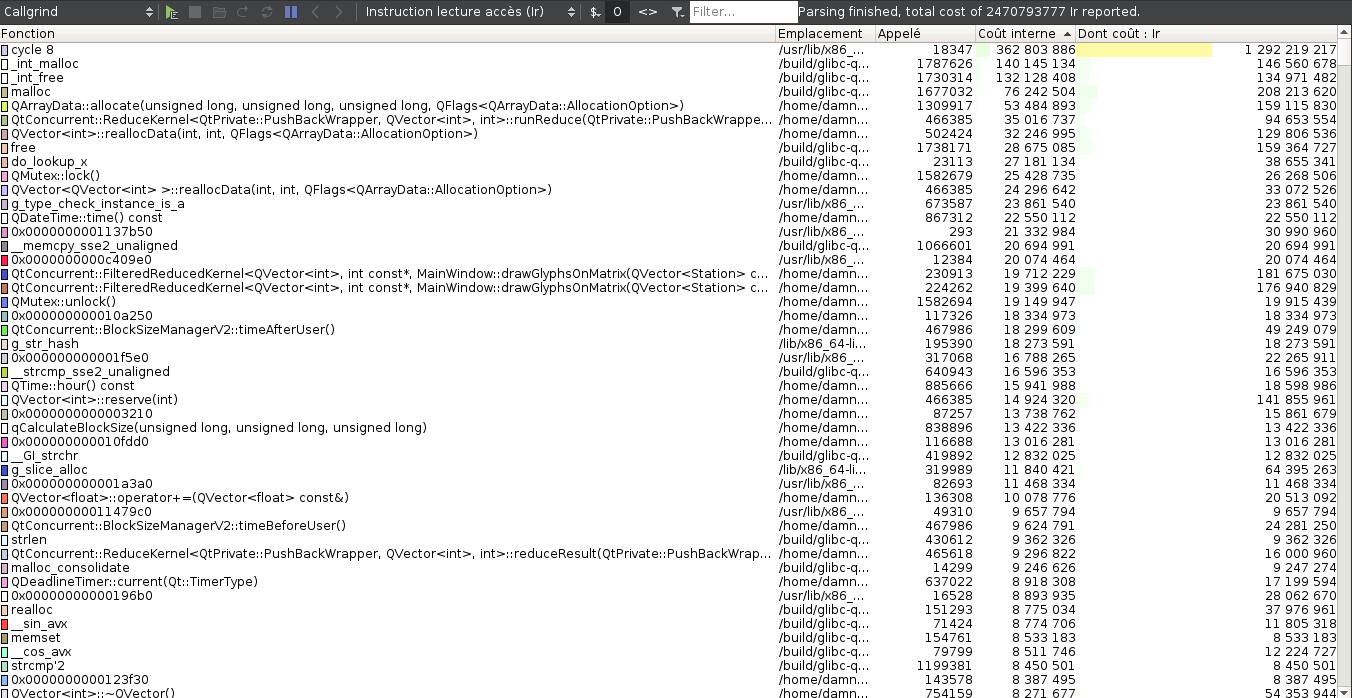
\includegraphics[scale=.38]{callgrind_analyse.png}
		\caption{Analyse de fonctions avec Callgrind}
		\label{fig:callgrind}
		\end{center}
		\end{figure}
	
		Pour réaliser cette analyse, nous avons compilé en mode “Release” afin d’avoir
		un code optimisé et le plus rapide possible à l’exécution.
		Sur cette analyse on peut voir que les fonctions les plus lourdes sont les fonctions
		parallélisées notamment \textit{drawGlyphsOnMatrix}. L’allocation des QVector<QVector<int>>
		prend aussi beaucoup de temps . On notera aussi QDateTime::time.
		
		\subsection{Fuite de mémoire}
		Nous avons testé les fuites de mémoire avec le programme Valgrind en utilisant la
		commande suivante:
	
		\begin{verbatim}	
		valgrind --leak-check=full ./VisualBSS
		\end{verbatim}
	
		\begin{figure}[!h]
		\begin{center}
		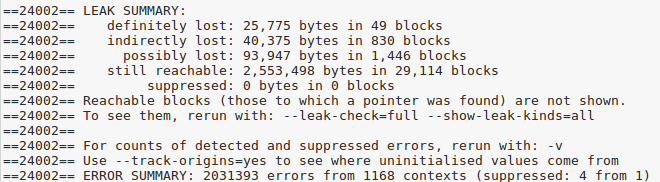
\includegraphics[scale=.8]{memory_leak.png}
		\caption{Tests de fuites de mémoire avec Valgrind}
		\end{center}
		\end{figure}	
	
		Lorsqu'on analyse avec \textit{Valgrind} les fuites de mémoire que notre application
		génère lors de la fermeture de l'application, l’intégralité des fuites
		générées sont propres au framework de Qt. Ces fuites sont malheureusement non
		supprimables.\\
		En revanche, nous n'avons pas trouvé de fuite de mémoire venant de notre code.\\
		
		Vous trouverez dans les annexes (cf: Figure \ref{fig:autres_exemples_fuites_memoire}) une
		impression écran avec des exemples de fuites mémoire que généré le programme.
	
\newpage
\part{Bilan}
	\section{Bugs présents}		
		\subsection{Sélection dans la timelinematrix}
		La sélection des heures et des stations se fait avec le rectangle bleu dessiné par
		l'utilisateur grâce à sa souris. Le problème vient des indices des stations qui
		sont incorrectes.
		La fonction \textit{MatrixGLWidget::stationIntervalSelected} renvoie de mauvaise valeurs
		. Jusqu'ici, par manque de temps, nous n'avons pas réussi à corriger l'erreur.
		
		\subsection{Courbes de Bézier}
		Il y a une erreur dans le calcul du point de contrôle, la courbe n'est pas parfaitement
		symétrique en son milieu.
		
	\newpage
	\section{Les difficultés rencontrées}
		\subsection{Compréhension du sujet et fonctionnalités}
		Pour réaliser ce projet nous devions nous appuyer sur le document rédigé par le groupe de
	chercheurs, ainsi que la vidéo. Pour réaliser notre cahier des besoins, il nous a été
	difficile de définir certains besoins car il nous manquait des informations ou précisions.
	De même pour l’application montrée dans la vidéo, nous ne pouvions pas la tester car nous
	n'avions pas accès.\\

	Concernant la réalisation de l’affiche avec OpenGL, nous somme resté bloqué plusieurs jours
	sur un bug. Le problème venait des identifiants que nous passions aux VBO. Ces identifiants
	était incorrecte et donc l'affichage était anarchique.
	Cela nous a fait perdre beaucoup de temps.\\

	Durant le phase de développement, nous avons perdu du temps également à cause de la
	stratégie à adopter pour stocker les trajets et les stations. Nous avons essayé de faire
	simple et performant. Cela nous a valu de changer le code et de faire des tests pour savoir
	si les performances étaient présente.
	
	
		\subsection{Implémentation du programme}
		Le projet est destiné à visualiser et traiter via des filtres une grande quantité de données (environ un million de trajets). Il est donc facile de rendre le programme peut interactif au niveau utilisateur ou de mal utiliser les ressources de mémoire vive.\\

Le point crucial, face à ce défi, a donc été de choisir correctement les structures de données pour représenter les trajets et stations, les prototypes de fonctions qui les manipulent, ainsi que l’utilisation du parallélisme. Cela a impliqué de devoir rechercher sur Internet des sujets (principalement StackOverflow, en complément de la documentation de Qt) qui traitent de l’efficacité des conteneurs ainsi que d’autres possibilités d’optimisations de construction, stockage et traitement de ces données.
		
		
		\subsection{Implémentation de l’interface graphique}	
		L’existant propose de filtrer les trajets et stations en manipulant des intervalles de valeurs, via des sliders à deux poignées. Qt propose ce genre de widget avec le module \textit{QtQuick}. Nous l’avons découvert relativement tard son existence, et cela nous a pris du temps pour comprendre comment l'intégrer. Nous avons ainsi perdu du temps à tenter d’implémenter en C++ ce widget, sans succès.\\
	
		Une fois son intégration réussie, un nouveau problème se posait : suite à un rendez-vous avec le client, nous avons découvert qu’il ne disposait pas du module nécessaire, et qu’il ne souhaitait pas l’installer. De plus, son comportement était instable, notamment lorsqu’on relâchait une poignée, elle revenait à sa position d’origine.\\
	
		Une solution a donc était d’utiliser une spinbox, un widget disponible dans le module \textit{Widget} de Qt, qui permet de réaliser les mêmes choses qu’un slider, à savoir modifier une valeur sur un intervalle. Chaque slider à deux poignées a donc été remplacé par deux spinbox.
	
	\newpage
	\section{Critiques et améliorations possible} \label{ameliorations}	
		\subsection{Représentation des données à afficher} 
		Un structure ou classe \textit{Vertex} aurait dû être implémentée, elle contiendrait un vecteur
		à 2 dimensions pour les positions 2D et un vecteur à 3 dimensions pour stocker les trois
		composantes rouge, vert et bleu.
		Dans notre cas,
		lors de la construction des données à afficher (calculs des positions et couleurs), nous
		mettons ces données représentées par des flottants, dans un \textit{QVector}.
	
		\subsection{Performances}
		Par rapport à l’existant, on s'aperçoit vite que le programme est mal optimisé, avec notamment un temps pour filtrer les trajets beaucoup trop long.\\
	
		L’architecture est en cause, notamment parce que le contrôleur entretient les identifiants des données, et que les fonctions de filtrage prennent en paramètre des données. Il faut ainsi récupérer les données à partir de leurs identifiants pour filtrer, et vice-versa (récupérer les données à partir de leurs identifiants) après filtrage. Cela est coûteux dans le sens où il faut itérer sur chacune des données, et allouer des conteneurs intermédiaires.\\
		
		Ainsi, pour exemple, le prototype de la fonction chargée de filtrer les trajets ne serait plus
\textit{QVector<Trip> TripsFilter::filter(QVector<Trip> trips)} serait remplacé par 
\textit{QVector<int> TripsFilter::filter(QVector<int> tripsIds, QVector<Trip> trips)}. Le premier prototype traite directement les trajets, tandis que le deuxième nécessite un accés indexé sur une lookup-table. La deuxième approche est moins élégante, mais améliorerait fortement l’efficacité des méthodes qui filtrer les trajets. Il en vaut de même pour les méthodes de filtrage et tri des stations, ainsi que sélection des trajets.\\
	
		Une solution consiste à faire en sorte que les fonctions de filtrage prennent en paramètre les identifiants des données à filtrer, ainsi que la table d’indexation des données. Ces fonctions retournent ainsi non plus des données mais les identifiants des données filtrées. Il n’y aurait donc plus d’opérations aussi coûteuses d’allocation de conteneurs intermédiaires.\\
	
		Une autre solution, qui changerait davantage l’architecture, serait d’oublier ce système d’indexation des données par leurs identifiants, et d’utiliser des pointeurs. Cela implique de parfaitement connaître le lieu (dans le code) et l’instant (à l'exécution) d’allocation des données, ainsi que le lieu et l’instant de leur désallocation, sous peine de provoquer des fuites mémoires.
	
		\subsection{Interactivité : sélection des glyphes}
		\textbf{A PRECISER}\\
		Les ralentissements que cela occasionne nous a contraint à réduire l’interactivité de
	notre application en mettant à jour les trajets sélectionnés dans la \textit{timelinematrix} qu’une
	fois que l’utilisateur ait relâché le bouton gauche de la souris.
		
		\subsection{Implémentation du contrôleur}
		La classe \textit{MainWindow}, qui joue le rôle de contrôleur, fait communiquer la vue et le modèle. Le problème est qu’elle accumule les fonctionnalités, donc les fonctions. Elle contient donc trop de fonctions et est difficilement maintenable et lisible (les bugs en témoignent ces problèmes).\\
	
		Pour l’instant, aucune solution n’a été pensée, bien que la solution proposée plus haut pour éviter les conversions données/identifiants des données supprimerait de nombreuses lignes de code, ainsi que deux fonctions.
		
		\subsection{Perspectives}
		Il serait tout à fait possible de reprendre l'article \ref{Oli16} afin d’étendre le programme
		en ajoutant d'autres modes de visualisations. Par exemple on pourrait afficher les stations
		qui serait vides ou pleines en fonction de l'heure de la journée. Bien sûr, il faudrait trouver
		les différentes sources de données permettant cela.
		
	\newpage
	\section{Conclusion}

	\newpage
	\section{Lexique}
	\begin{itemize}
		\item[]\textbf{BSS} : bike sharing system, système de vélos en libre service\\
		\item[]\textbf{CSV} : CSV : Comma Separated Value, c'est un format de fichier\\
		\item[]\textbf{XML} : Extensible Markup Language, c'est un langage de balisage.\\
		\item[]\textbf{JSON} : Java Script Object Notation, format de fichier\\
		\item[]\textbf{Qt} : Est un framework très populaire pour le développement
		d'interfaces graphiques\\
		\item[]\textbf{Valgrind} : framework permettant de faire de l'analyse de programmes\\
		\item[]\textbf{Tests en boites blanche} : Testes qui visent à regarder l’implémentation même 
		des fonctions, contrairement aux tests boites noire, on regarde le fonctionnement des objets.\\
		\item[]\textbf{Test en boite noire} : Vise tester le comportement de l'application et nom pas 
		les objets ou fonctions.\\
		\item[]\textbf{Doxygene} : Outil permettant de générer de la documentation,
		au format html ou en Latex par exemple.\\
		\item[]\textbf{Glyphe} : Un glyphe est un élément de la \textit{timelinematrix}, elle
		représente un ensemble de trajet d'une station donnée est d'une heure donnée.\\
		\item[]\textbf{Shared pointer} :\\
		\item[]\textbf{Parsing} : Analyse d'une chaîne de symboles.\\
		\item[]\textbf{QML} : Qt Modeling Language\\
		\item[]\textbf{OpenGL} : Ensemble de fonctions permettant d'écrire des applications graphique.
		Elle est disponible sous de nombreuses plateformes comme Linux, Windows ou MacOS par exmple.
		\item[]\textbf{GLSL} : OpenGL Shader Language, langage pour écrire des Shaders avec OpenGL\\
		\item[]\textbf{Shader} : C'est un programme écrit en GLSL (proche du langage C), qui sera
		exécuté par la carte graphique.\\
	\end{itemize}
	
	\newpage
	\bibliography{bibliographie}	
	
	\newpage
	\section{Annexes}
		\subsection{Génération de courbes de Bézier (code)}	\label{code_courbes_bezier}
		
		\lstset{language=C++,
		                basicstyle=\ttfamily,
		                keywordstyle=\color{blue}\ttfamily,
		                stringstyle=\color{red}\ttfamily,
		                commentstyle=\color{green}\ttfamily,
		                morecomment=[l][\color{green}]{\#}
		}
		\begin{lstlisting}
		vec3 evalQuadraticBezier(vec3 v[3], float t)
		{
		    float oneMinusT = 1.0 - t;

		    float b0 = oneMinusT * oneMinusT;
		    float b1 = 2.0 * oneMinusT * t;
		    float b2 = t * t;
		    
		    return b0 * v[0] + b1 * v[1] + b2 * v[2];
		}
		\end{lstlisting}
		
		Cette fonction GLSL evalue la position du nouveau en fonction de la position des 3
		points de contrôle ainsi que de t, l'intervalle sur laquelle on se trouve.\\
		
				\lstset{language=C++,
		                basicstyle=\ttfamily,
		                keywordstyle=\color{blue}\ttfamily,
		                stringstyle=\color{red}\ttfamily,
		                commentstyle=\color{green}\ttfamily,
		                morecomment=[l][\color{green}]{\#}
		}
		\begin{lstlisting}
		vec3 pos[3];
	    pos[0] = gl_in[0].gl_Position.xyz;
	    pos[1] = posCP;
	    pos[2] = gl_in[1].gl_Position.xyz;
	
	    float pointsInterval = 1.0 / float(generatedPointsNb - 1.0);
	
	    for(int i = 0; i < generatedPointsNb; i++)
	    {
	        float t = i * pointsInterval;
	        vec3 p = evalQuadraticBezier(pos, t);
	
	        gl_Position = vec4(p.xyz, 1.0);
	
	        // color interpolation
	        gColor = mix(vColor[0], vColor[1], t);
	
	        EmitVertex();
	    }
	
	    EndPrimitive();
		\end{lstlisting}
		
		Ceci est une partie du code se trouvant dans la fonction \textit{main} du geometry shader. \\
		A chaque itération de la boucle \textit{for}, un nouveau est généré.\\
		
		\clearpage
	
		\subsection{Comparatif du nombres de points généré}	 \label{comparatif_courbes_bezier}		
		\begin{figure}[!h]
		\begin{center}
		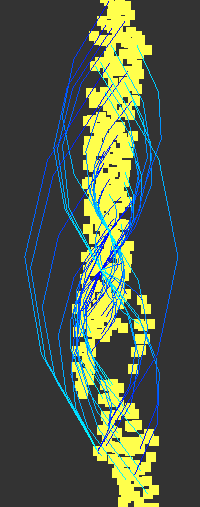
\includegraphics[scale=.60]{5_generated_points.png}
		\caption{Courbes de Bézier avec 5 points généré}
		\end{center}
		\end{figure}
		
		\begin{figure}[!h]
		\begin{center}
		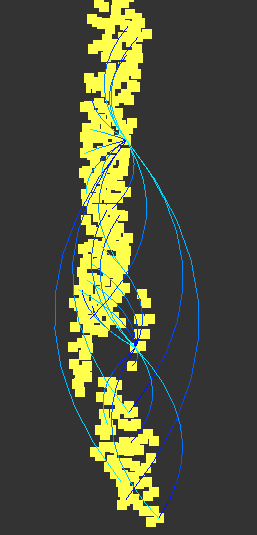
\includegraphics[scale=.60]{10_generated_points.png}
		\caption{Courbes de Bézier avec 10 points généré}
		\end{center}
		\end{figure}
		
		\begin{figure}[!h]
		\begin{center}
		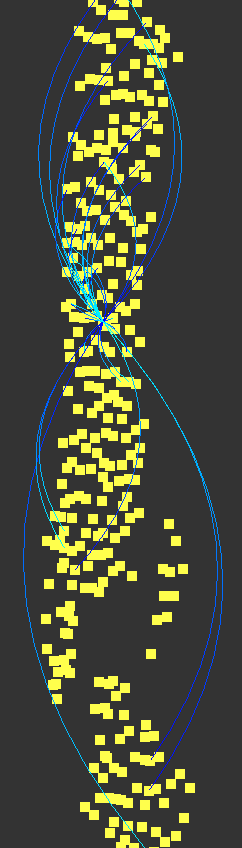
\includegraphics[scale=.60]{15_generated_points.png}
		\caption{Courbes de Bézier avec 15 points généré}
		\end{center}
		\end{figure}
		
		\begin{figure}[!h]
		\begin{center}
		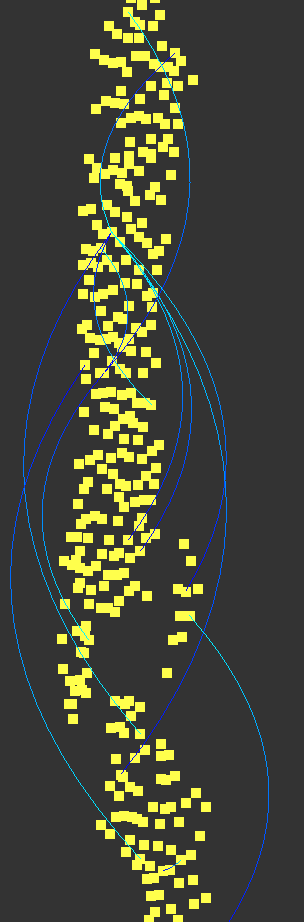
\includegraphics[scale=.60]{20_generated_points.png}
		\caption{Courbes de Bézier avec 20 points généré}
		\end{center}
		\end{figure}
		
		\begin{figure}[!h]
		\begin{center}
		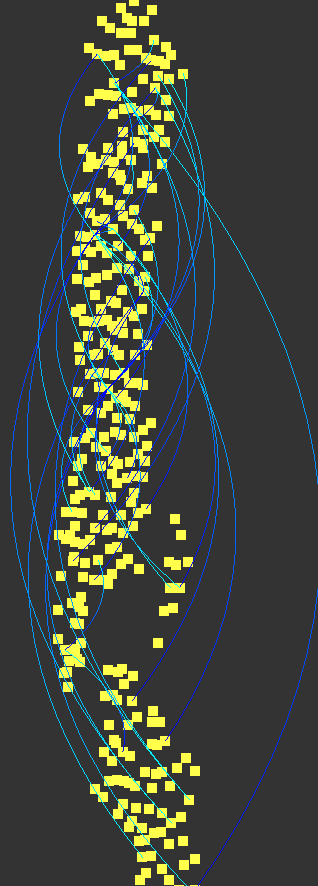
\includegraphics[scale=.60]{25_generated_points.png}
		\caption{Courbes de Bézier avec 25 points généré}
		\end{center}
		\end{figure}
		\clearpage
				
		
		\subsection{Sortie Valgrind (fuites de mémoire)}
		\begin{figure}[!h]
		\begin{center}
		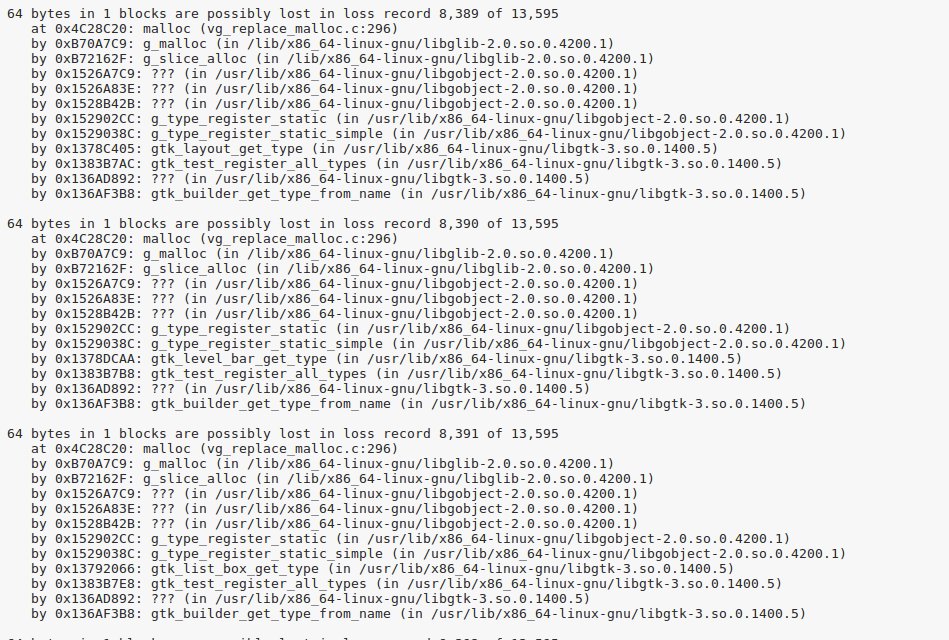
\includegraphics[scale=.60]{autres_exemple_fuites_memoire.png}
		\caption{Autres exemples de fuites de mémoire avec Valgrind}
		\label{fig:autres_exemples_fuites_memoire}
		\end{center}
		\end{figure}
		
		\clearpage		
		
		\subsection{Manuel utilisateur}
 
\end{document}